
%%%%%%%%%%%%%%%%%%%%%%%%%%%%%%%%%%%%%%%%%%%%%%%%%%%%%%%%%%%%%%%%%%%%%
%% This is a (brief) model paper using the achemso class
%% The document class accepts keyval options, which should include
%% the target journal and optionally the manuscript type.
%%%%%%%%%%%%%%%%%%%%%%%%%%%%%%%%%%%%%%%%%%%%%%%%%%%%%%%%%%%%%%%%%%%%%
\documentclass[journal=iecred,manuscript=article]{achemso}

%%%%%%%%%%%%%%%%%%%%%%%%%%%%%%%%%%%%%%%%%%%%%%%%%%%%%%%%%%%%%%%%%%%%%
%% Place any additional packages needed here.  Only include packages
%% which are essential, to avoid problems later. Do NOT use any
%% packages which require e-TeX (for example etoolbox): the e-TeX
%% extensions are not currently available on the ACS conversion
%% servers.
%%%%%%%%%%%%%%%%%%%%%%%%%%%%%%%%%%%%%%%%%%%%%%%%%%%%%%%%%%%%%%%%%%%%%
\usepackage[version=3]{mhchem} % Formula subscripts using \ce{}
\usepackage[T1]{fontenc}       % Use modern font encodings

\usepackage{amsmath, amsthm, amsfonts}
\usepackage{caption}
\usepackage{subcaption}
\usepackage{csquotes}
\usepackage{multirow}
% Theorems
%-----------------------------------------------------------------
\newtheorem{thm}{Theorem}[section]
\newtheorem{cor}[thm]{Corollary}
\newtheorem{lem}[thm]{Lemma}
\newtheorem{prop}[thm]{Proposition}
\newtheorem{exem}{Example}
\theoremstyle{definition}
\newtheorem{defn}[thm]{Definition}
\theoremstyle{remark}
\newtheorem{rem}[thm]{Remark}
\newcommand{\fim}{ \hfill{\mbox{$\rule{2mm}{2mm}$}}\vskip.6cm }

% Shortcuts.
% One can define new commands to shorten frequently used
% constructions. As an example, this defines the R and Z used
% for the real and integer numbers.
%-----------------------------------------------------------------
\def\RR{\mathbb{R}}
\def\ZZ{\mathbb{Z}}


%%%%%%%%%%%%%%%%%%%%%%%%%%%%%%%%%%%%%%%%%%%%%%%%%%%%%%%%%%%%%%%%%%%%%
%% If issues arise when submitting your manuscript, you may want to
%% un-comment the next line.  This provides information on the
%% version of every file you have used.
%%%%%%%%%%%%%%%%%%%%%%%%%%%%%%%%%%%%%%%%%%%%%%%%%%%%%%%%%%%%%%%%%%%%%
%%\listfiles

%%%%%%%%%%%%%%%%%%%%%%%%%%%%%%%%%%%%%%%%%%%%%%%%%%%%%%%%%%%%%%%%%%%%%
%% Place any additional macros here.  Please use \newcommand* where
%% possible, and avoid layout-changing macros (which are not used
%% when typesetting).
%%%%%%%%%%%%%%%%%%%%%%%%%%%%%%%%%%%%%%%%%%%%%%%%%%%%%%%%%%%%%%%%%%%%%
\newcommand*\mycommand[1]{\texttt{\emph{#1}}}

%%%%%%%%%%%%%%%%%%%%%%%%%%%%%%%%%%%%%%%%%%%%%%%%%%%%%%%%%%%%%%%%%%%%%
%% Meta-data block
%% ---------------
%% Each author should be given as a separate \author command.
%%
%% Corresponding authors should have an e-mail given after the author
%% name as an \email command. Phone and fax numbers can be given
%% using \phone and \fax, respectively; this information is optional.
%%
%% The affiliation of authors is given after the authors; each
%% \affiliation command applies to all preceding authors not already
%% assigned an affiliation.
%%
%% The affiliation takes an option argument for the short name.  This
%% will typically be something like "University of Somewhere".
%%
%% The \altaffiliation macro should be used for new address, etc.
%% On the other hand, \alsoaffiliation is used on a per author basis
%% when authors are associated with multiple institutions.
%%%%%%%%%%%%%%%%%%%%%%%%%%%%%%%%%%%%%%%%%%%%%%%%%%%%%%%%%%%%%%%%%%%%%
\author{G. B. Libotte}
\author{F. D. Moura Neto}
\altaffiliation{Instituto de Matem\'atica Pura e Aplicada, Rio de Janeiro, Brazil}
%\altaffiliation{Current address: Some other place, Othert\"own,
%Germany}
% \alsoaffiliation[Second University]
% {Instituto de Matemática Pura e Aplicada, Rio de Janeiro, Brazil}
\author{L. F. C. Jatob\'{a}}
\author{C. N. Parajara}
\author{G. M. Platt}

%\altaffiliation{A shared footnote}
%\email{i.k.groupleader@unknown.uu}
\phone{+55 (22)25192166}
%\fax{+123 (0)123 4445557}
\affiliation[Unknown University]
{Polytechnic Institute, Rio de Janeiro State University, Nova Friburgo, Brazil}
%\alsoaffiliation[Second University]
%{Department of Chemistry, Second University, Nearby Town}
%\author{Susanne K. Laborator}
\email{gmplatt@iprj.uerj.br}
%\affiliation[BigPharma]
%{Lead Discovery, BigPharma, Big Town, USA}
%\author{Kay T. Finally}
%\affiliation[Unknown University]
%{Department of Chemistry, Unknown University, Unknown Town}
%\alsoaffiliation[Second University]
%{Department of Chemistry, Second University, Nearby Town}

%%%%%%%%%%%%%%%%%%%%%%%%%%%%%%%%%%%%%%%%%%%%%%%%%%%%%%%%%%%%%%%%%%%%%
%% The document title should be given as usual. Some journals require
%% a running title from the author: this should be supplied as an
%% optional argument to \title.
%%%%%%%%%%%%%%%%%%%%%%%%%%%%%%%%%%%%%%%%%%%%%%%%%%%%%%%%%%%%%%%%%%%%%
\title[An \textsf{achemso} demo]
  {Geometry of Double Retrograde Vaporization Prediction}

%%%%%%%%%%%%%%%%%%%%%%%%%%%%%%%%%%%%%%%%%%%%%%%%%%%%%%%%%%%%%%%%%%%%%
%% Some journals require a list of abbreviations or keywords to be
%% supplied. These should be set up here, and will be printed after
%% the title and author information, if needed.
%%%%%%%%%%%%%%%%%%%%%%%%%%%%%%%%%%%%%%%%%%%%%%%%%%%%%%%%%%%%%%%%%%%%%
\abbreviations{IR,NMR,UV}
\keywords{American Chemical Society, \LaTeX}

\graphicspath{{Pictures/}} % Specifies the directory where pictures are stored

%%%%%%%%%%%%%%%%%%%%%%%%%%%%%%%%%%%%%%%%%%%%%%%%%%%%%%%%%%%%%%%%%%%%%
%% The manuscript does not need to include \maketitle, which is
%% executed automatically.
%%%%%%%%%%%%%%%%%%%%%%%%%%%%%%%%%%%%%%%%%%%%%%%%%%%%%%%%%%%%%%%%%%%%%
\begin{document}

%%%%%%%%%%%%%%%%%%%%%%%%%%%%%%%%%%%%%%%%%%%%%%%%%%%%%%%%%%%%%%%%%%%%%
%% The "tocentry" environment can be used to create an entry for the
%% graphical table of contents. It is given here as some journals
%% require that it is printed as part of the abstract page. It will
%% be automatically moved as appropriate.
%%%%%%%%%%%%%%%%%%%%%%%%%%%%%%%%%%%%%%%%%%%%%%%%%%%%%%%%%%%%%%%%%%%%%
\begin{tocentry}

Some journals require a graphical entry for the Table of Contents.
This should be laid out \enquote{print ready} so that the sizing of the
text is correct.

Inside the \texttt{tocentry} environment, the font used is Helvetica
8\,pt, as required by \emph{Journal of the American Chemical
Society}.

The surrounding frame is 9\,cm by 3.5\,cm, which is the maximum
permitted for  \emph{Journal of the American Chemical Society}
graphical table of content entries. The box will not resize if the
content is too big: instead it will overflow the edge of the box.

This box and the associated title will always be printed on a
separate page at the end of the document.

\end{tocentry}

%%%%%%%%%%%%%%%%%%%%%%%%%%%%%%%%%%%%%%%%%%%%%%%%%%%%%%%%%%%%%%%%%%%%%
%% The abstract environment will automatically gobble the contents
%% if an abstract is not used by the target journal.
%%%%%%%%%%%%%%%%%%%%%%%%%%%%%%%%%%%%%%%%%%%%%%%%%%%%%%%%%%%%%%%%%%%%%
\begin{abstract}
 Double retrograde vaporization is a phase behavior phenomenon 
 that occurs close to the critical point of binary mixtures. 
 Here we employ sophisticated modern numerical methodology to 
 untangle the geometry of this complex phenomenon, based on the
 robust methodology of inversion of funtions.
 ..........
\end{abstract}

%%%%%%%%%%%%%%%%%%%%%%%%%%%%%%%%%%%%%%%%%%%%%%%%%%%%%%%%%%%%%%%%%%%%%
%% Start the main part of the manuscript here.
%%%%%%%%%%%%%%%%%%%%%%%%%%%%%%%%%%%%%%%%%%%%%%%%%%%%%%%%%%%%%%%%%%%%%
\section{Introduction}

Double retrograde vaporization is a phase behavior phenomenon that occurs close to the critical point of binary mixtures, that is, the point where there are no phase boundaries and therefore the distinction between them does not exist, causing the mixture to cease to exist as well. It occurs in mixtures characterized by involving a solvent with high volatility relative to the solute contained in the mixture. More specifically in relation to the mixture to be studied, composed of ethane + limonene, the solvent boils at 184.6 K, while the boiling point of the solute is 448.2 K. This tendency towards evaporation of ethane in relation to limonene causes its volatility to be high, satisfying one of the conditions of occurrence.

The phenomenon corresponds to a special shape of the dew-point curve, exhibiting a \enquote{S} shape (with three dew points) or a double-dome structure (with four dew points), for specific system temperature and composition. Especially in the case of double-dome manifestation, the phenomenon occurs within a very limited temperature range, which is slightly above to the critical temperature of the more volatile component. We must mention that the composition of vapor phase is arbitrarily chosen, in order to produce the thermodynamic phenomenon.

Its occurrence was firstly investigated by \citet{chen_1} and \citet{chen_2} for binary mixtures involving methane + n-butane and methane + n-pentane, under specified temperature. More recently, \citet{raeissi_1} identified a double-dome behavior for the binary mixture ethane + limonene at $T = 307.4$ K and in a narrow range of compositions (close to the pure ethane). Furthermore, \citet{raeissi_2} indicated that the Peng-Robinson equation of state \citep{peng_robinson}, with classical mixing rules, was capable to qualitatively predict this phenomenon. In order to detail the thermodynamic fundamentals of double retrograde vaporization, \citet{raeissi2004thermodynamic} also presented a detailed discussion of the volumetric properties of the fluids involved as defining the existence of the phenomenon.

In the vicinity of the mixture critical point, the robust calculation of dew point pressures (under specified temperature) is a very hard task. Furthermore, some roots of the phase equilibrium problem show very small radius of convergence for Newton-type methods, as indicated by \citet{jnsa}. For this reason, the development of robust frameworks for this type of problem is extremely relevant. Among several possibilities, we focus on the robust methodology of the numerical inversion of functions, proposed by \citet{malta}, 
where they developed an extensive theory to handle functions
in a generic class of functions
defined in the whole plane to the plane. 
Their theory give precise statements about the 
solution of 2 by 2 systems of nonlinear equations, when 
the function is defined everywhere in the plane. 
From their theory we select a few techniques which
are applicable to our thermodynamic problem, namely, this technique \citep{malta} proposes --- considering a 
generic class of functions --- the computation of
 critical curves in the mathematical 
sense\footnote{The term \enquote{critical} assumes two meanings in this work: in the mathematical sense, a critical point of a function
 is a nonregular point (where the Jacobian matrix is 
 non-invertible); in the thermodynamic sense, the 
 critical point is that where we cannot distinguish 
 between the properties of the phases.}, the construction 
 of a bank of solved points
  (to be used  as 
 with good initial estimates for all 
 the possibly multiple solutions) and, finally, the inversion 
 of the desired point (calculation of all pre-images of a such 
 image).
 
As far as we know, the first application of these techniques of the general methodology of numerical inversion of functions from the plane to the plane, adapting them to handle a chemical engineering problem, was presented by \citet{canadian}, in the prediction of the azeotropic behavior in systems with double azeotropes. More recenlty, \citet{ireme} presented some preliminary results regarding the application of the methodology proposed by \citet{malta} in the prediction of double retrograde vaporization phenomenon in the system ethane + limonene.

In addition to being a robust framework in the resolution of nonlinear systems, the method of inversion of functions from the plane to the plane provides relevant information that allows a deeper analysis of the function studied. Some aspects are fundamental for understanding the behavior of the function from a global perspective. Among these aspects, we can briefly mention: (i) the influence of the system temperature in the critical curves, and (ii) the analysis of the behavior of inversions near the critical image (where the number of pre-images --- solutions of the system --- change). 
As pointed previously, the solution of this kind of nonlinear system with typical derivative based root-finding algorithms
 (such as Newton's methods) is not a trivial task, even when using more sophisticated numerical tools \cite{jnsa} and thus,
 one of the objectives of this work is to provide a 
 geometrical view of this challenging nonlinear algebraic system, which can be useful in the development of numerical tools for solving high-pressure phase equilibrium problems. 

In order to analyze these main points and provide an in-depth 
geometric study of the phase equilibrium problem in two-component systems, we present two case studies.
The first one is the system composed of ethane + limonene at 
$ T = 307.4 $ K which is analyzed, fixing the molar fraction of the vapor phase of ethane at $ y_{1} = 0.998966 $.
 Under these conditions, the system presents four distinct solutions,
corresponding to the intersections of the dew point curve 
with the line of a given mole fraction, as can be seen in 
Figure \ref{fig:dew_point_curve}. For this system, all the
 steps of the method of inversion of functions from the plane 
 to the plane were performed and the solution degeneration was 
 investigated by obtaining pre-images of a set of points 
 located in the vicinity of the critical image. We also 
 evaluated the critical points of the 
function that defines the nonlinear system 
that are folds and cusps, and their relation with the degeneration of solutions of this problem.

\begin{figure}
	\begin{center}
		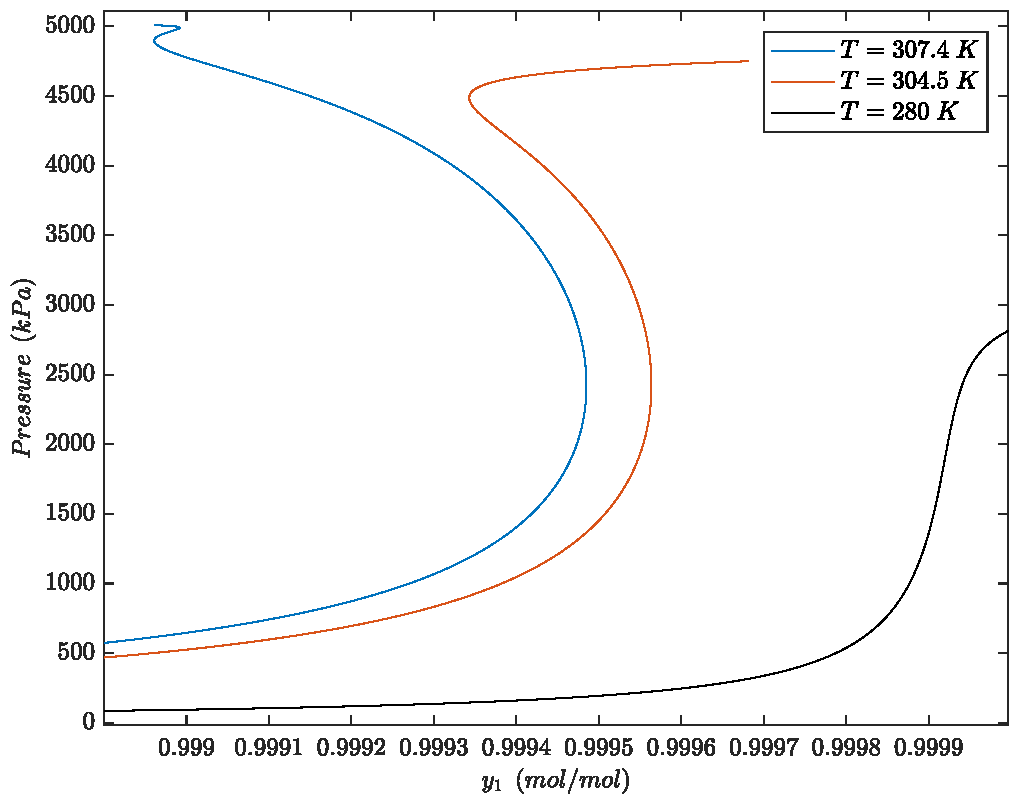
\includegraphics[scale=0.50]{curvas_ponto_orvalho.pdf}
		\caption{Dew point curves for the system ethane + limonene at several temperatures.}\label{fig:dew_point_curve}
	\end{center}
\end{figure}

In the second case study,  the temperature of the system 
composed of the same components of the previous case was set at  $ T = 304.5 $ K and compared 
 with the same system at $T = 280$ K. In these temperature
 scenarios, with $ y_1 = 0.99945 $ (among other conditions), the system has
  three and one solutions, respectively, as shown in Figure \ref{fig:dew_point_curve}. Thus, it is
   possible to evaluate the degeneracy of solutions in both systems, varying only one of the parameters of the problem.

The possibility of solving the problem --- and therefore obtaining the pre-images of a given point in the image --- was also evaluated from a mathematical perspective: the critical curves 
of the function defining  the nonlinear
 system were obtained for different temperatures and their respective critical images. Through this variation, for a 
 fixed molar fraction of ethane in the vapor phase, it was possible to verify the influence of the critical curves in obtaining the solutions of the problem through methods that use derivatives.

 The remaining of this work is organized as follows. First we
 discuss the thermodynamic model. Next we 
 present the mathematical 
 and numerical methodology, beginning with an example of 
 a scalar function of one variable (1D case) and 
 showing how the critical points and their images are used
 to break the equation in cases where the number of 
 solutions is constant, followed by  a discussion of functions
 of two variables (2D case),
  and fold and cusp critical points. The 
 construction of the critical set and 
 of the bank of solved problems is next. Finally we present
 and discuss 
 the numerical examples, and conclusions.

\section{Models and Methodology}

\subsection{Thermodynamic models and problem formulation}

All the phase equilibrium calculations, as well as the critical point curves (in the thermodynamic sense), are
 conducted for the Peng-Robinson equation of state with classical mixing rules and null binary interaction parameters. Critical properties and acentric factors of pure components can be found, for instance, in \citet{ireme}.

For a binary mixture, the phase equilibrium problem can be formulated as:
\begin{eqnarray}
\hat{\phi}_i^L x_i = \hat{\phi}_i^V y_i\:, \hspace{0.1in} i = 1,2\:.
\end{eqnarray}
In the last equation, $\hat{\phi}$ represents the fugacity coefficient for component $i$ (using the Peng-Robinson model), $x_i$ is the molar fraction in the liquid phase and $y_i$ represents the vapor phase. The superscripts $L$ and $V$ refer to the liquid and vapor phases, respectively.

Using $x_2 = 1 - x_1$ and $y_2 = 1 - y_1$, the nonlinear algebraic problem (in the plane) is then:
\begin{subequations} \label{eq:sistema_problema}
\begin{eqnarray}
\hat{\phi}_1^L x_1 = \hat{\phi}_1^V y_1\:, \\
\hat{\phi}_2^L (1-x_1) = \hat{\phi}_2^V (1-y_1)\:.
\end{eqnarray}
\end{subequations}

The vector of unknowns, considering the specification of temperature and vapor molar fractions, is $p = (x_1,\;P)$. Let the residue of the nonlinear equations be denoted by $f_i$, and define  $F =F(x_1,\;P)=(f_1,\;f_2)= (\hat{\phi}_1^L x_1 - \hat{\phi}_1^V y_1,\;\hat{\phi}_2^L (1-x_1) - \hat{\phi}_2^V (1-y_1))$. 
Thus, in general, the nonlinear algebraic system can be re-stated as
%
\begin{equation}
F(p) = q\: ,
\end{equation}
where $p$ is a point in the domain and $q$ is a point in the 
image (range) of $F$. Ordinarily, we are interested to 
solve $F(p) = (0,0)$ (where $q=(0,0)$ represents the null
 vector in the Euclidean plane).

\subsection{Some features of the numerical 
 inversion of 
functions}
Here we present a few fundamental ideas on the solution 
of a nonlinear system by numerical inversion of the
associated functions.
\subsubsection{An 1D example}
To get a grasp of the methodology of inversion of functions to 
solve nonlinear systems of equations, we first consider a 
simple 1D example.
Let $F(p)=p^3-3p^2+ 2p=p(p-1)(p-2)$. 
Assume that for physical reasons $p$ is always non-negative.
By examining the graph of $F$ it is possible to 
check that the equation for $q$,
\begin{eqnarray*}
F(p)=q, \ \ \text{that is}, \ p^3-3p^2+ 2p=q\ ,
\end{eqnarray*}
has  0 to 3 solutions. If $\eta(q)$ denotes the 
number of solutions as a function of $q$, then, 
\begin{small}
\begin{eqnarray*}
\eta(q)= \left\{ 
\begin{array}{rl}
0 , & \text{if } q< -2\sqrt{3}/9\\
1, & \text{if } q= -2\sqrt{3}/9 \text{ or } q > 2\sqrt{3}/9\\
2 , & \text{if }  -2\sqrt{3}/9 < q  < 0 \\
3 , & \text{if } 0\leq q< 2\sqrt{3}/9
\end{array}\: .
\right.
\end{eqnarray*}
\end{small}
The jumping points, where 
 the number of solutions can change, are either the
 image of a critical point --- a critical image ---
 or an image of a boundary point of the domain of definition
 of $F$.
  The critical points
(where the derivative is zero) satisfy
\begin{eqnarray*}
F'(p)=3p^2-6p+2 = 0, \ \text{that is } p=1 \pm \sqrt{3}/3\ .
\end{eqnarray*}
Since 0 is the only boundary point of the domain,
 the jumping points are 
$F(1 \pm \sqrt{3}/3)=\mp 2\sqrt{3}/9$ and $F(0)=0$.  
%
These  points suggest  a partition of the
 range of $F$  in seven subsets, 
$\text{I\!R}= {\cal T}_1\cup {\cal J}_2\cup {\cal T}_3 \cup {\cal J}_4 \cup {\cal T}_5\cup {\cal J}_6\cup {\cal T}_7$,
%
\begin{equation*}
\begin{split}
\text{jumping sets} \quad & {\cal{J}}_{2} = \left\lbrace-\frac{2\sqrt{3}}{9}\right\rbrace , \; {\cal{J}}_{4} = \left\lbrace 0 \right\rbrace , \; {\cal{J}}_{6} = \left\lbrace\frac{2\sqrt{3}}{9}\right\rbrace \\
\text{tile sets} \quad & {\cal{T}}_{1} = \left] -\infty,\;-\frac{2\sqrt{3}}{9}\right[ , \; {\cal{T}}_{3} = \left] -\frac{2\sqrt{3}}{9}, \; 0\right[ , \; {\cal{T}}_{5} = \left]0, \; \frac{2\sqrt{3}}{9}\right[ , \; {\cal{T}}_{7} = \left]\frac{2\sqrt{3}}{9}, \; +\infty\right[ \\
\end{split}
\end{equation*}

\noindent Note that the number of solutions is constant in each tile. The overall strategy for solving the equation $F(p)=q$ is to compute the jumping sets and, by taking the complementary set, decompose the range of $F$ in its jumping and tile sets, have a bank of solved points with representatives more or less covering all the tile sets, and to solve the equation with the bank of solved points providing initial guesses for each solution.
%

\subsubsection{Jumping and tiles in the 2D case}
Now we consider 2$\times$2 systems of  equations, $F(p)=q$, 
with 
$q\in \text{I\!R}^2$ and $F$ a function defined on a 
subset $\Omega$ 
of  the plane to the plane, 
$F:\text{I\!R}^2\supset \Omega\to \text{I\!R}^2$. Recall 
that  
the Jacobian $JF|_p$ at a point $p=(x,y)\in \text{I\!R}^2$ is
%
\[ JF|_p  = \begin{pmatrix}
\dfrac{\partial f_1}{\partial x} & \dfrac{\partial f_1}{\partial y} \vspace{0.5em} \\
\dfrac{\partial f_2}{\partial x} & \dfrac{\partial f_2}{\partial y}
\end{pmatrix} \; . \]

\noindent A point $ p $ in the domain is said  a critical 
point if $ JF|_p $ is not invertible, which is equivalent to 
say that $ \det\left(JF|_p\right) =0 $.
A critical point is non-degenerate if
  $ \text{grad}\left(\det\left(JF|_p\right)\right) \neq 0 $.
 Under such conditions, the Jacobian matrix is not the null 
 matrix. Therefore, this matrix has rank equal to one in $ p $ 
 and there is a nonzero vector that is tangent to the critical 
 curve. As a consequence, 
if a function has only non-degenerate critical points
--- which we assume --- their set 
is formed by curves, the
critical curves, 
\begin{eqnarray*}
{\cal C}= \{p\in \text{I\!R}^2 \mid \det(JF|_q)=0\}\ ,
\end{eqnarray*}
and the image of ${\cal C}$, 
$F({\cal C})=\{q=F(p), \text{ for all } p \in {\cal C}\}$, is
called  
the critical image. 
The set formed by the union of the
critical image and the image of the 
boundary of the domain of $F$, ${\cal J}=F({\cal C})\cup F(\Omega)$, define the jumping curves. The tiles 
are the connected components on the complement of $\cal J$; 
if there are $k$ connected components, ${\cal T}_i$, 
then $\text{I\!R}^2= \left( \cup_{i=1}^k{\cal T}_i\right) \cup{\cal J}$, just as in the 1D example.
The number of solutions of the equation $F(p)=q$
is constant if $ q\in {\cal T}_i$, and may jump when crossing  ${\cal J}$.


One of the drawbacks to the application of the detailed 
theory 
presented in 
\citet{malta} to problems coming from applications 
that involve the solution of nonlinear $2\times 2$ systems of 
equations
is not so much that it applies only to a special collection of
functions, but that the functions have to be defined 
in all points in the plane. When that happens, 
the theory gives a fairly good amount
of information on the solutions of the nonlinear system of 
equations.
In applications, however,  the domain of a function has to
satisfy some 
restrictions due, for instance, to the lack of physical
 significance
of certain values of the variables,
 or due to existence of singularities, 
which breaks the theory presented in \citet{malta}.
This is the case in the problems we are considering
since, {\em e.g.}, the volume cannot be less than a certain 
quantity,
and the pressure cannot be above certain critical value.
 Nonetheless
the overall methodology that they discuss is preserved 
in the form of algorithms.

\subsubsection{The inversion of functions from the plane to the plane}
Next, we present 
the method of inversion of functions from the plane to 
the plane,  as well as the main definitions 
that support the technique. A detailed description of the 
method can be found in \citet{malta}.

The method is intended to solve systems with two equations and
 two unknowns of type $ F\left(p\right) = q $ with $ p, q \in 
{\text{I\!R}}^2 $ and $ F $ should be a smooth function. In dealing specifically with critical points, they are assumed of just two types, either folds or cusps. 
% Before addressing each of them, it is important to introduce that a point in the image of $ F $ is called a regular value if all of its pre-images are regular points, as previously defined. 
A fold is a non-degenerate critical point such that:
%
\begin{itemize}
\item the kernel $ K $ of the Jacobian and the tangent line $ T $ to the critical set in $ p $ do not coincide.
\end{itemize}

In cases where the kernel $ K $ and the line $ T $ tangent to the critical set coincide, there is a cusp-like critical point. In general,  cusps are non-degenerate critical points such that:
%
\begin{itemize}
\item the kernel $ K $ of the Jacobian and the tangent line $ T $ to the critical set in $ p $ coincide;
\item for a smooth parametrization $ \gamma : \left( -\epsilon, \; \epsilon \right) \to {\text{I\!R}}^2 $ of $ C $ near $ p $, with $ \gamma \left(0\right) = p $ and $ \gamma^{\prime} \left(0\right) \neq 0 $, the angle $ \theta\left(\gamma\left(t\right)\right) $ between the kernel $ K\left(\gamma\left(t\right)\right) $ of $ J\left(\gamma\left(t\right)\right) $ and the tangent line $ T\left(\gamma\left(t\right)\right) $ to $ C $ satisfies $ \theta^{\prime}\left(0\right) \neq 0 $.
\end{itemize}

Within the scope of  functions from the plane to the plane, we 
must introduce two descriptions of very important type of 
functions. 
A continuous function from a subset of the plane to the plane 
is proper if  $\lim_{\vert\left(x,\;y\right)\vert\to\infty} \vert F\left(x,\;y\right)\vert = \infty$. This avoids to
treat equations with infinitely many solutions. A 1D case, of an equation with infinite solutions, is $\sin x=0$. This happens because $\sin x$ is not a proper function. 
%
In turn, a smooth proper function from the plane into itself is excellent if every critical point of $ F $ is a fold or a cusp. In essence, the theory developed in \citet{malta} aims
at solving equations defined by excellent functions that 
satisfy yet another technical condition, the nice 
functions. For them, the theory 
asserts several results. 
An essential feature of the class of nice functions 
is that, under a suitable topology, they are generic
in a mathematical sense.
That means in particular
that they are an open set. From a simplified point of view, 
that property expresses that any smooth
function can be approximated arbitrarily close by a nice function. 
 Therefore,
the analysis can be restricted to this type of function.
That is, in practice, it is enough to work 
with nice functions, thus the critical points are only 
cusps and folds.


% algorithm was constructed to solve the $ 2\times2 $ nonlinear system of algebraic equations $ F\left(p\right) = q $, when $ F:{\text{I\!R}}^2 \to {\text{I\!R}}^2 $ is a nice function. Let $ F $ be an excellent and proper function. It is nice if its critical set $ C $ is limited and the critical image $ F\left(C\right) $ consists of a normal family of curves. $ F\left(\gamma\right) $  is a normal curve when there are no points with more than two pre-images in $ \gamma $ and, at points of self-intersection, the vectors tangent to $ F\left(\gamma\right) $ are linearly independent.

% Faced with this fact, one of the difficulties is to apply the method of inversion of functions from te plane to the plane in engineering problems. The complexity in parameterizing functions that describe this type of problem and checking the properties and theorems that underlie the method are some of the difficulties. At the outset, the task of verifying whether the functions describing the mathematical model of a particular engineering problem is nice can be complex. 


The methodology of inversion of functions from
a subset of the plane to the plane is composed of three 
fundamental steps: obtaining the critical set of $ F $, 
creating the bank of solved points and calculating the pre-images from an arbitrary point. Each of these steps will be described next.

\subsubsection{Generation of the critical set}

Knowing the critical set is fundamental in the inversion process, since it 
allows the computation of the critical image which, as
illustrated in the 1D example, are places where the number
of solutions can change --- in these cases  we say that the 
solutions
degenerate.
 In addition to tracing the regions where the continuation method does not face points of singularity in the inversion process, it also indicates the boundary
 of the  different tiles, which is a primordial concept in the analysis of solution degeneration. 

In the original procedure, \citet{malta} proposes various calculations and verifications in order to establish that, strictly speaking, the critical points obtained form the critical set as a whole. In addition, the computational routine still sorts the critical points and locates points of intersection of the curves in the image. Due to the difficulties mentioned above regarding the application of the technique to solve real engineering problems, some adaptations were made to the original method, so that it could be simplified without affecting its main attributes.

Initially, the problem domain is fully mapped. An equally spaced rectangular mesh is constructed in the domain of the problem and the value of the determinant of the Jacobian matrix at each point is calculated. Since the critical points are those in which the determinant of the Jacobian is null, the mesh is traversed, and each time changes 
  in the signal of the determinant are identified,
   an arbitrary point of the segment between the two points 
   of the mesh with distinct signals is taken as initial guess of the root calculation.
    Therefore, a Newton-type routine is executed until the critical point within the segment of the mesh
     is obtained.

The previous procedure is executed until all the mesh is traversed, that is, until all the critical points of the domain are obtained, forming the critical set. 
 The mesh must be sufficiently refined so that the
 whole set of  critical curves can be obtained,
  with the desired accuracy. After obtaining the set $ {\cal C} $ of critical curves, the set of critical images 
  $F\left({\cal C}\right) $ follows by calculating the value of the function of each of the critical points contained in $ {\cal C} $.

\subsubsection{Creation of the bank of solved points}
The bank of solved points is a set of points in the image 
where all their respective pre-images in the 
domain are known since they have been carefully 
computed. 
These points are then used as initial guesses for the process 
of inversion of an arbitrary point in the image of the 
function. The bank of solved points can be as extensive as desired and obtaining the pre-images of each of the points can be performed by the continuation method (when at least one
pre-image is known)
 or by using a numerical method capable of getting the whole set $ p_{a} $ when $F\left(p_{a}\right) = q_{a} $.
Since the inversion method can fail if it approaches sufficiently close to the critical set, it is instrumental the  creation of a bank of solved points, 
 to effectively be able to solve the system of equations
 in general.
  It is a set of points in the image where all their respective pre-images in the domain are known. 

Once  the bank of solved points has been built,
 it is needed to adopt an appropriate criteria in choosing the point that is  used as the beginning point in the path 
 created by the continuation method. Originally, the technique adopts different criteria based on the following properties: the calculated segments in the inversion process should stay away from critical points, especially from  the 
 cusp type, which are difficult to obtain pre-images. In addition, the segments should have few intersections with $ F\left({\cal C}\right) $, due to the possible degeneration of solutions. Also, segments should be as short as possible. However, due to difficulties the criterion assumed for the choice of the bank point that will be taken as the initial guess of the continuation process in the inversion step is the calculation of the shortest path, since the critical points are not classified in the step of obtaining the critical curves and it is intended to avoid that the segment crosses the critical curve. In this way, the point $ q_{0} $ of the bank with the least Euclidean distance in relation to $ q $ --- the point to be inverted --- is chosen.

Choosing the point that will generate the shortest path does not guarantee that the segment will not cross some critical curve. If $ q_{0} $ is located on a different tile than $ q $, the inversion process may have problems, since the segment will necessarily cross some image of a critical or boundary curve before $ q $ is reached. Therefore, it is convenient that the bank of solved points be formed by points contained in different tiles, according to the problem solving requirements.

From the point of view of user interference in relation to each of the steps of the method, the creation of the bank of solved points is the most expensive stage, especially when they are very extensive and there are several
 pre-images, according to each specific problem. However, the homotopy-continuation technique used in the inversion step (see more in \citet{allgower}) allows the use of a single bank in solving different problems of the same genre, that is, with variation of parameters, as shown in \citet{canadian}, which solved the double azeotropy problem of the system composed of benzene + hexafluorobenzene at different values of the system pressure, with the same bank of solved points generated at $ P = 20 \; kPa $.
 
\subsubsection{Inversion of an arbitrary point}

The calculation of the pre-images is accomplished through the creation of L-shaped paths using the Euler-Newton continuation method. Initially, the element $ q_{0} $ of the bank of solved points in the image that is closest to the point to be inverted $ q $ is selected. Then, the points are connected to each other through two perpendicular segments, joined by their ends, going from $ q_{0} $ to $ q $, which produces an intermediate point, called $ \tilde{q} $. The respective path in the domain will be traversed through the continuation method, starting from $ p_{0} $, that is, the point of the bank of solved points in the domain referring to $ q_{0} $. Since each point of the image stored in the bank must have all of its respective pre-images also kept in the bank, the inversion step must be executed as many times as there are entries stored in the bank of solved points in the domain relative to $ q $, in order that all the solutions of the system are found, producing different L-shaped paths, which start from the same initial guess.

The predictor-corrector method used to trace the L-shaped path is based on homotopy techniques. 
%
%Here, only the main points of the methodology will be treated.
%
In a rudimentary way, take $ F:\text{I\!R}^{n} \to \text{I\!R}^{n} $ a smooth map. In an attempt to find the values of $ p $ that determine the solutions of $ F\left(p\right) - q = 0 $, numerical methods may fail when no prior knowledge of $ F $ is known and the initial guesses taken may not be good enough to solve the problem. One way to avoid this kind of problem is to deform the original function through a homotopy technique and try to trace an implicitly defined curve in order to reach the solution of the system through a starting point.
%
%Therefore, the homotopy $ H:\text{I\!R}^{n}\times\text{I\!R} \to \text{I\!R}^{n} $ is a smooth map. One can choose the convex homotopy, which is given by
%
%\[ H \left( p,\; \lambda \right) = F \left( p \right) - \lambda q - \left( 1 - \lambda \right) q_{0} \; , \]
%
%\noindent where $ q $ is the point in the image to be inverted, $ q_{0} $ is the point of the bank of solved points that will be taken as the initial guess in an attempt to trace an implicitly defined curve and $ \lambda $ is a real parameter, such that $ \lambda \in \left[ 0, \; 1 \right] $. Note that the original problem can be retrieved when $ \lambda $ assumes the extreme values of the range in which it is defined.

%The purpose of the predictor-corrector method is to trace the curve by varying the $ \lambda $ value over the interval in which it is defined, generating a sequence of points and respecting a given tolerance.
%
The scheme used in the continuation method employs the Euler's method in the predictor step and, in turn, the Newton's method is responsible for the refinement of the predicted solution in the corrector step.
%This method obtains the point sequence that approaches the curve through the recurrence relation
%
%\[ v_{i + 1} = u_{i} + ht \left( H^{\prime}\left( u_{i} \right) \right) \; , \]
%
%\noindent where $ h > 0 $ represents the stepsize and $ t \left( H^{\prime}\left( u_{i} \right) \right) $ is an unitary vector tangent to the solution curve at the point $ u_{i} $, obtained by QR decomposition. The stepsize must be arbitrarily small in order to obtain a reasonable approximation. Also, if $ u_{i} $ is sufficiently close to the curve, then the predicted point $ v_{i + 1} $ will also be sufficiently close to the curve and the minimization problem will have an unique solution, which will be refined in the corrector step. In turn, the scheme used in the corrector step is the Newton's method.
%However, the jacobian matrix $ H^{\prime} $ is not square, since the homotopy technique introduces the $ \lambda $ parameter into the function that describes the problem, and therefore the matrix is not invertible. Thus, Newton's method requires modifications to satisfy the dimension of the problem. Therefore, the problem of minimization motivates the introduction of an alternative to the inversion of non-square matrices: the Moore-Penrose inverse. Denoted by $ A^{+} $, the Moore-Penrose right inverse of a matrix $ A $ is defined by $ A^{+} = A^{T} \left(AA^{T}\right)^{-1} $, where $ A $ is a $ n \times \left( n + 1 \right) $ matrix with maximal rank. Therefore, the recurrence relation that defines Newton's method in the corrector step is given by
%
%\[ w_{i + 1} = v_{i + 1} - H^{\prime}\left(v_{i + 1}\right)^{+} H\left(v_{i + 1}\right) \; . \]
%
After calculating a point that approximates the curve of interest in each of the iterations of the predictor-corrector method, %through the approach mentioned above
a stepsize adaptation strategy is adopted for the next iteration. It is convenient to adopt strategies of this type to avoid regions that contain singularities or to prevent the numerical method from making big jumps during the calculation of the curve. Using this artifice, it is also possible to perform a complementary evaluation of the convergence of the method. Details about method implementation will not be described here. All information about the computational routines used in the inversion step can be found in \citet{allgower}.
%Thus, the first parameter of evaluation is the contraction rate of the corrector step, defined by the quotient of the Euclidean norm of two successive iterations of the Newton method. The stepsize should be adjusted if the sequence of contraction rate values are not decreasing.
%
%The stepsize can also be adjusted by analyzing the angle between two consecutive iterations, that is, the slope of the segment formed by subsequent points. By setting nominal values, one can define the appropriate stepsize for each of the iterations by analyzing these parameters. With this, the continuation method is subject to a \enquote{deceleration factor}, which varies between predefined limits. The details of the methodology will be omitted and can be viewed at \citet{allgower}.

\section{Numerical Results}

The methodology of numerical inversion of two-variable functions, adapted from \citet{malta} which considered the special case of functions from the plane to the plane, is employed in this phase equilibrium calculation. Some details regarding the construction of the bank of solved points and the numerical steps of the inversion process are given by \citet{ireme}. We present an in-depth analysis of the quantity of pre-images in limit-situations (for instance, when  the critical image is approached). Furthermore, we present the thermodynamic calculation of the critical points for the binary mixture ethane + limonene for the entire range of compositions. It will also be discussed the relation of the system temperature variation with the mathematical critical curves and the possibility of using a single bank of solved points for the resolution of several different systems.

As already mentioned, the results that will be presented here were obtained essentially from systems (as described in Equation \ref{eq:sistema_problema}) with three different configurations. In the first case, when the temperature of the system is $ T = 307.4 $ K and the molar fraction in the vapor phase of the ethane is set at $ y_{1} = 0.998966 $, the limit situation of inversion of a point arbitrarily close to the critical image will be evaluated and the degeneracy condition solutions will be analyzed. Under these conditions, some peculiar aspects about critical curves will also be shown. Furthermore, the degeneracy of solutions will also be examined from the point of view of the simultaneously resolution of two systems with different temperatures, in order to explain the disappearance of solutions under critical conditions. For this analysis, the system temperatures $ T = 304.5 $ K and $ T = 280 $ K will be taken, so that the molar fraction of ethane in the vapor phase is the same in both systems.
 
Table \ref{tab:resultados_pontos_orvalho_pressoes} presents the compositions and pressures for the dew point calculation in the system ethane + limonene at $T = 307.4$ K and $y_{1} = 0.998966 $, where the \enquote{double-dome} structure appears, with four dew point pressures (and compositions of the liquid phase), as shown in Figure \ref{fig:dew_point_curve}. The table also lists the results obtained by the method of inversion of functions from the plane to the plane for the phase equilibrium calculation problem when $ T = 304.5 $ K and $ T = 280 $ K, both fixed $ y_{1} = 0.99945 $, where a \enquote{S} shape dew curve appears, with three and one physical roots, respectively.

\begin{table}
\centering
\renewcommand*{\arraystretch}{1.3}
\caption{Dew point compositions and pressures for all cases studied.}
\label{tab:resultados_pontos_orvalho_pressoes}
\begin{tabular}{ccccccc}
\hline
\multirow{3}{*}{Roots} & \multicolumn{2}{c}{$ T = 307.4 $ K} & \multicolumn{2}{c}{$ T = 304.5 $ K} & \multicolumn{2}{c}{$ T = 280 $ K} \\
 & \multicolumn{2}{c}{$ y_{1} = 0.998966 $} & \multicolumn{4}{c}{$ y_{1} = 0.99945 $} \\ \cline{2-7} 
 & $ x_{1} \left( mol / mol \right) $ & $ P \left( kPa \right) $ & $ x_{1} \left( mol / mol \right) $ & $ P \left( kPa \right) $ & $ x_{1} \left( mol / mol \right) $ & $ P \left( kPa \right) $ \\ \hline
1 & 0.1567 & 619.3 & 0.3064 & 1209.4 & 0.0736 & 175.4 \\
2 & 0.9829 & 4859.5 & 0.8442 & 3900.9 & --- & --- \\
3 & 0.9918 & 4931.2 & 0.9917 & 4671.6 & --- & --- \\
4 & 0.9979 & 5007.3 & --- & --- & --- & --- \\ \hline
\end{tabular}
\end{table}

One can note that considering the data of the first case presented in Table \ref{tab:resultados_pontos_orvalho_pressoes}, that one solution corresponds to a low pressure root (root 1) and the others are high pressure roots (which are close to each other). From the point of view of the calculation techniques --- using classical numerical methods, such as Newton-Raphson methods --- we are interested in robust methodologies capable not only to find all roots, but also to find  the high pressure roots in a robust way. In order to better understand the geometry of the non-algebraic system of equilibrium, we consider some modified problems (perturbed versions of the original one) --- which bear no immediate physical meaning --- and use the same numbering of the roots (1 to 4).
 
\subsection{Thermodynamic critical point calculations}

Here we present the critical curve for the mixture ethane + limonene for the entire range of compositions. As reported previously, the term \enquote{critical curve} can exhibit two different meanings: the mathematical  and the thermodynamic.
 Here we deal
 with thermodynamic critical points, and we use the approach of Heidemman and Khalil \citep{heidemman}, with a double-loop structure in temperature-molar volume, for the critical point calculation.
 
\begin{figure}
	\begin{center}
		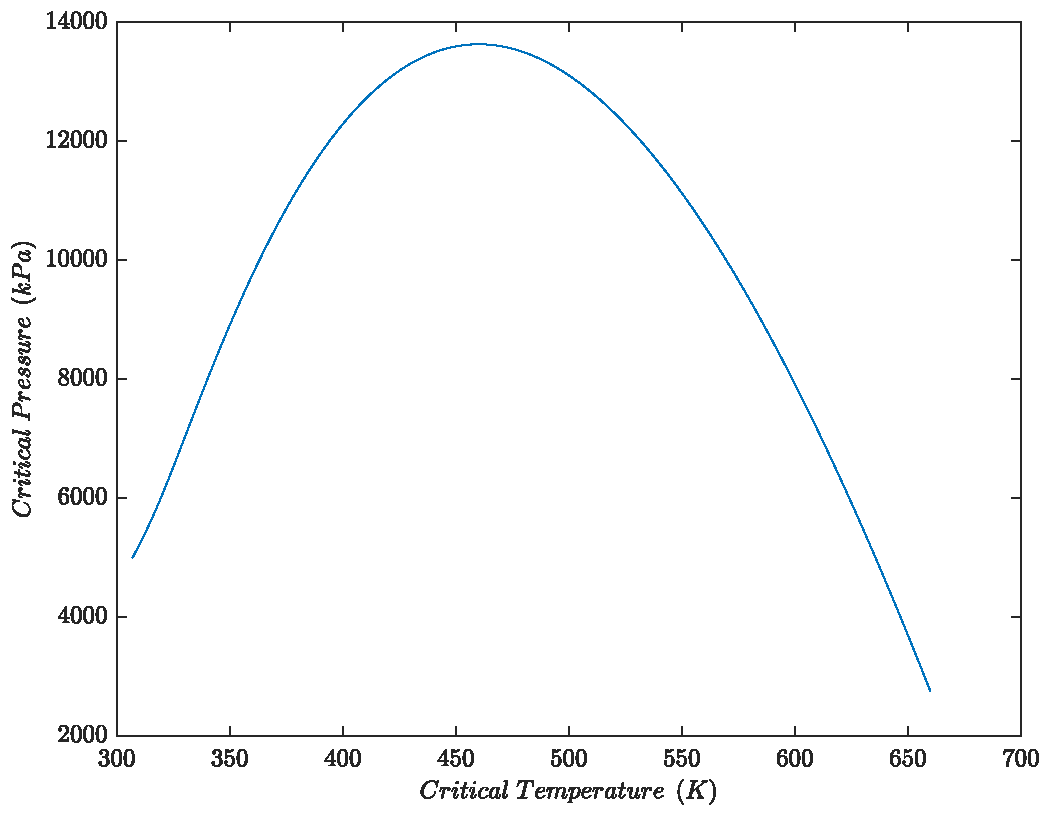
\includegraphics[scale=0.50]{temperatura_pressao.pdf}
		\caption{The thermodynamic critical curve in the system ethane + limonene.}\label{fig:critical_thermo}
	\end{center}
\end{figure}

Figure \ref{fig:critical_thermo} illustrates the critical curve, in the temperature-pressure plane, for the mixture at hand. We observe a continuous and unique curve connecting the two pure components. Thus, this system can be classified as Type I, accordingly to the classification of binary mixtures of Van Konynenburg and Scott \cite{classif}.

\subsection{Results at $T = 307.4 $ K and $y_1 = 0.998966$}

\subsubsection{An in-depth examination of the critical curves}

Here, we present a deeper analysis of the mathematical critical curves in this system. Clearly, we note that --- in the highlighted region --- the critical curves exhibit one self-intersection, as exhibited in Figure \ref{fig:sinais}. Furthermore, the two critical curves show a \enquote{quasi-tangent} point (or a meeting point).

\begin{figure}
	\begin{center}
		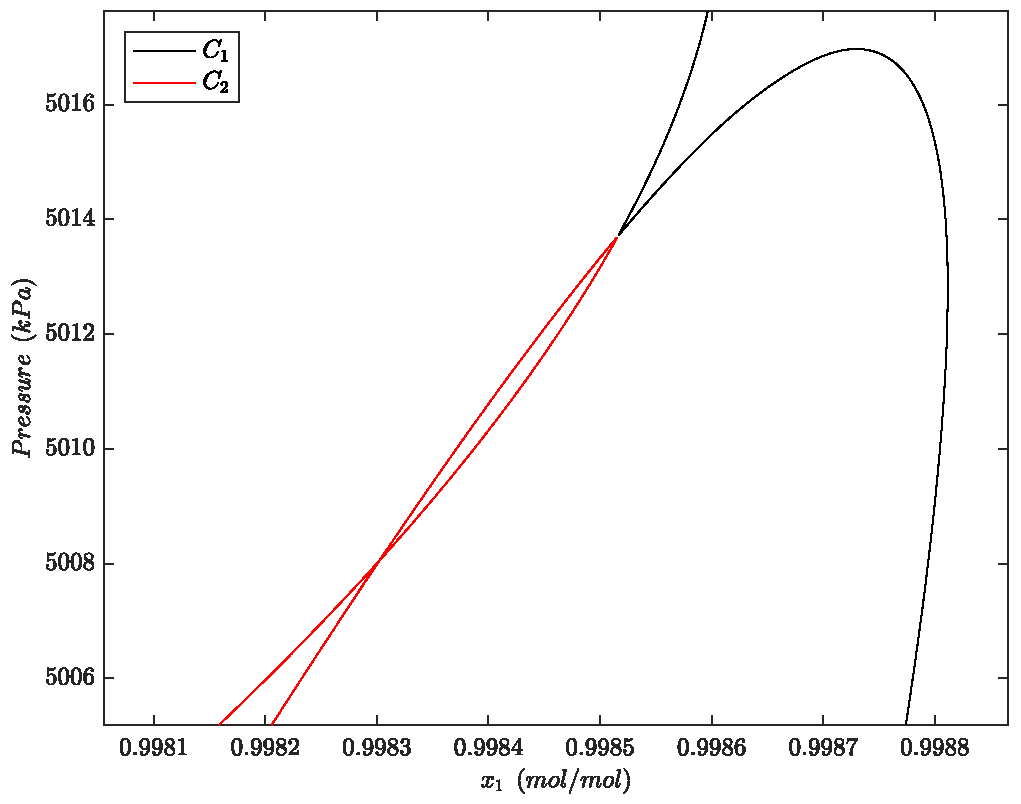
\includegraphics[scale=0.50]{curvas_criticas_dominio_new.pdf}
		\caption{A detailed view of the critical curves.}\label{fig:sinais}
	\end{center}
\end{figure}
 
\noindent An amplification of the region in the neighborhood of the \enquote{quasi-tangent} point, using a color pattern (in order to clarify the relationship between domain and image) is presented in Figure \ref{fig:domain_image}.

\begin{figure}
\centering
\begin{subfigure}{.5\textwidth}
  \centering
  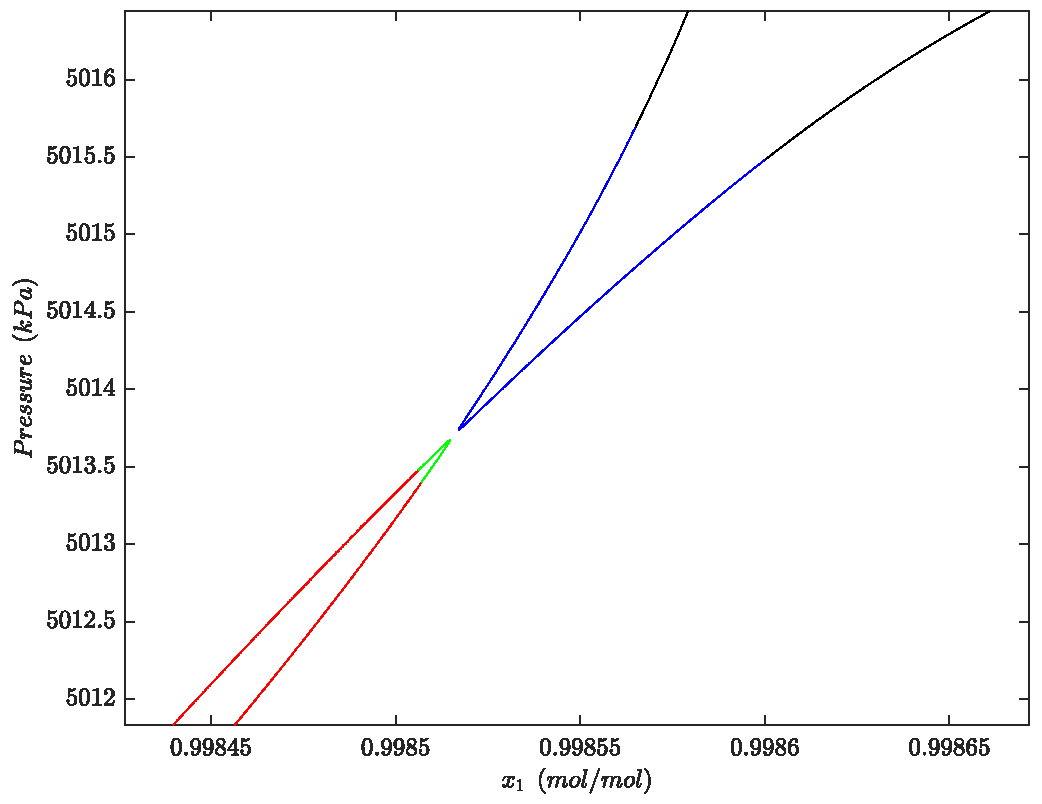
\includegraphics[width=.9\linewidth]{bicos_dominio}
  \caption{Domain}
  \label{fig:sub1}
\end{subfigure}%
\begin{subfigure}{.5\textwidth}
  \centering
  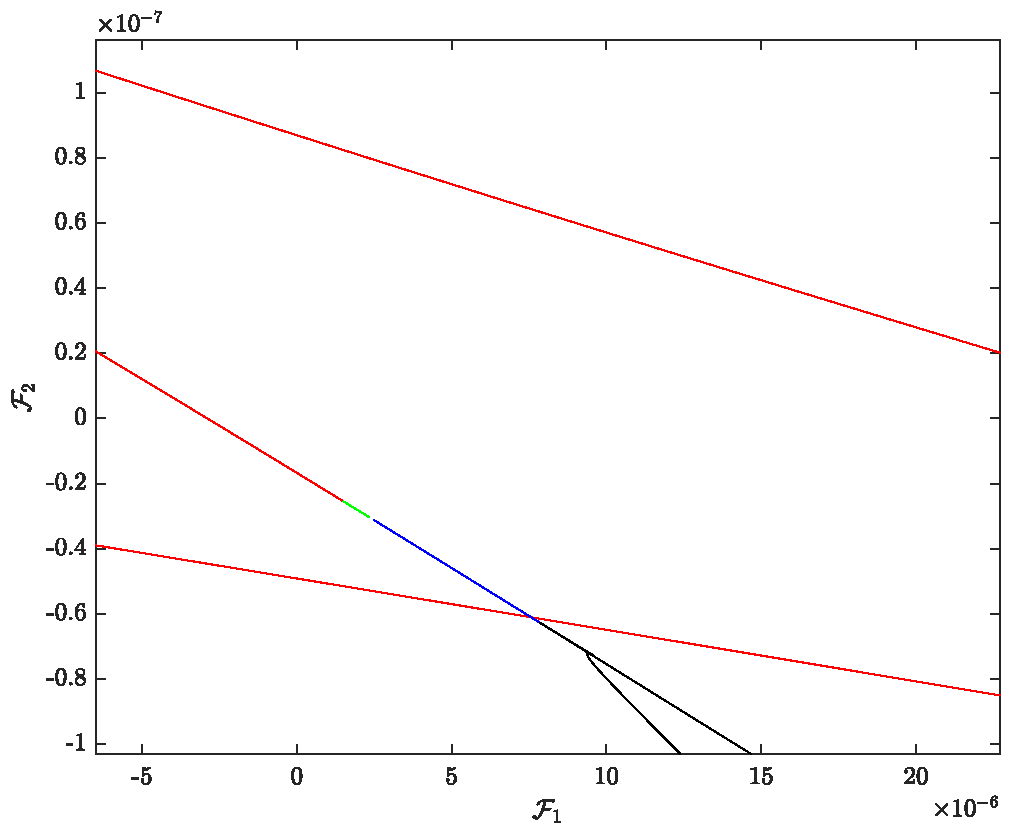
\includegraphics[width=.9\linewidth]{bicos_imagem}
  \caption{Image}
  \label{fig:sub2}
\end{subfigure}
\caption{Amplification of the interest region of the critical curve and the critical image.}
\label{fig:domain_image}
\end{figure}

\subsubsection{Inversion process --- approaching to the critical image}

Since the mathematical critical curves represent the set of points at which the value of the determinant of the Jacobian matrix is equal to zero, it is expected that the numerical method may have problems approaching these curves continuously until the degeneracy condition occurs, that is, a change in the quantity of their pre-images --- and therefore the solutions of the problem --- because of the collapse of solutions at a certain point in the critical curve. This occurrence helps to explain some cases of divergence of numerical methods based on derivatives.

Due to the nonlinearity of the problem, all the pre-images of a set of points in the image were obtained through the method of inversion of functions from the plane to the plane. The set of points in the image were arranged from $ q = \left(0,0\right) $ to a point sufficiently close to the critical image, equally spaced from each other and displaced only in the horizontal direction. In addition, each of the points in the image was identified by one color and their respective pre-images received the same color for all four sets of solutions mentioned above. Through this scheme, it was possible to analyze the behavior of the solutions in the domain and to estimate how close a pre-image of a given point $ q $ in the image approaches a critical curve, as $ q $ approaches the critical image.

\begin{figure}[!ht]
\centering
\begin{subfigure}{.48\textwidth}
  \centering
  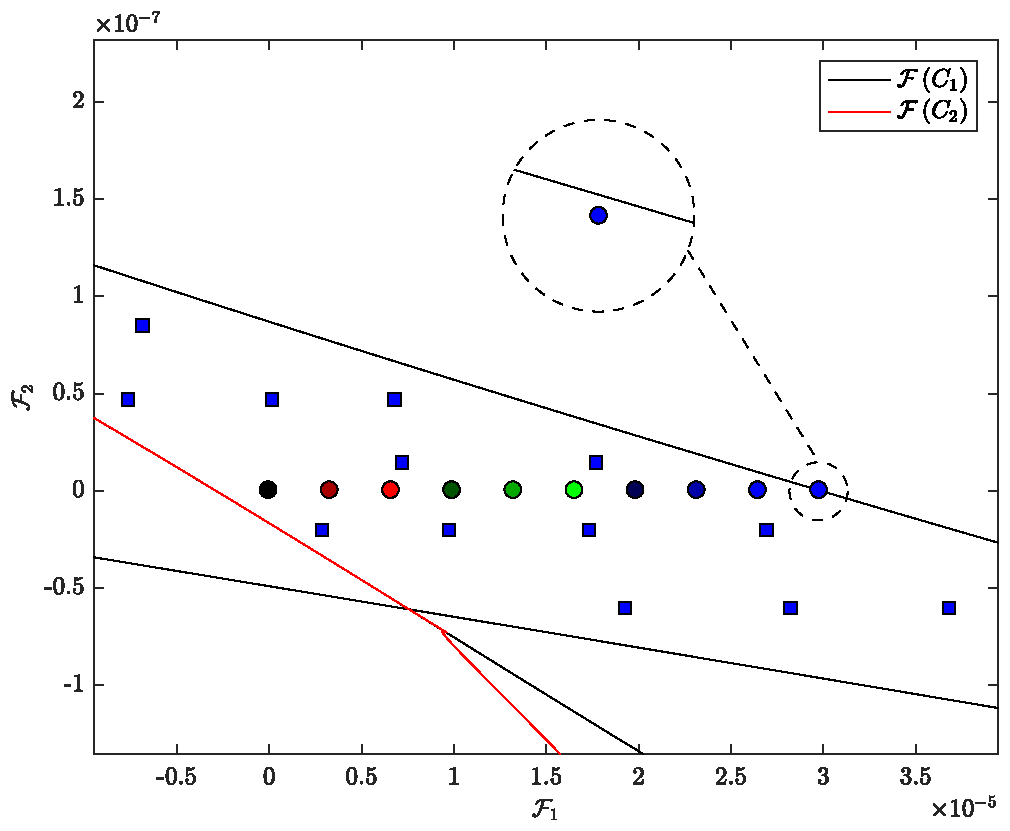
\includegraphics[width=\linewidth]{sequencia_pontos_imagem.pdf}
  \caption{Sequence of inverted points in the image.}
  \label{fig:points_image}
\end{subfigure}\hfill
\begin{subfigure}{.48\textwidth}
  \centering
  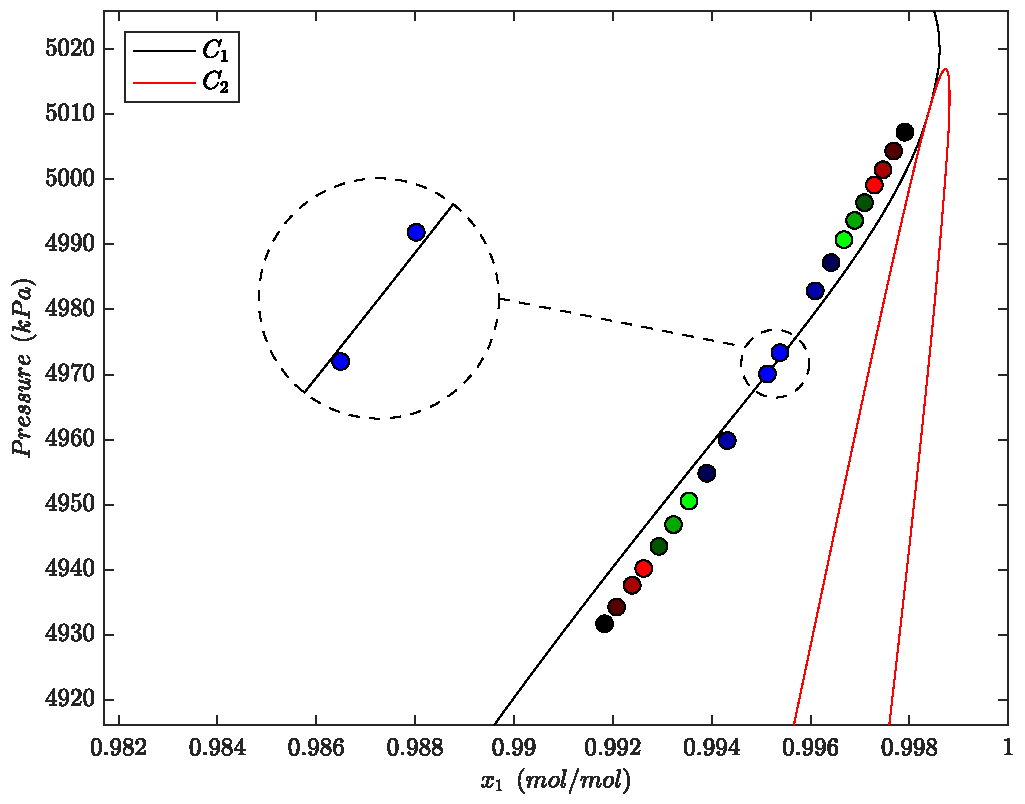
\includegraphics[width=\linewidth]{sequencia_pontos_dominio.pdf}
  \caption{Sequences of inverted points in the domain for roots 3 and 4.}
  \label{fig:points_domain_3_4}
\end{subfigure}\\
\begin{subfigure}{.48\textwidth}
  \centering
  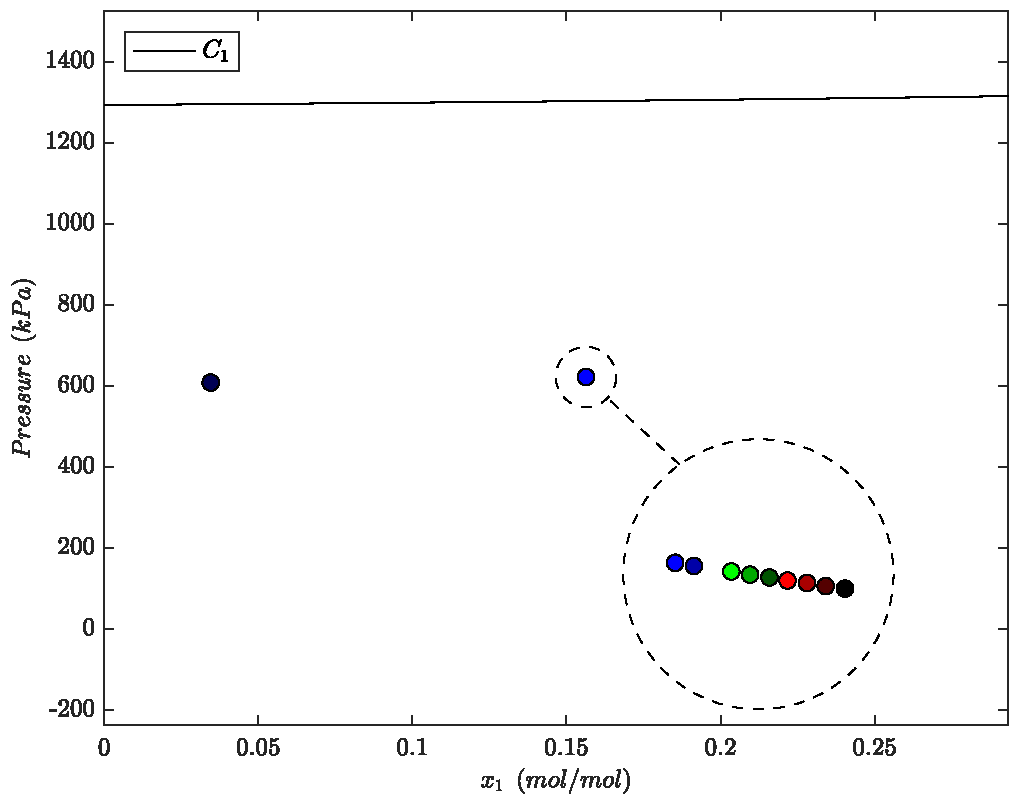
\includegraphics[width=\linewidth]{sequencia_pontos_dominio_3.pdf}
  \caption{Sequence of inverted points in the domain for root 1.}
  \label{fig:points_domain_1}
\end{subfigure}\hfill
\begin{subfigure}{.48\textwidth}
  \centering
  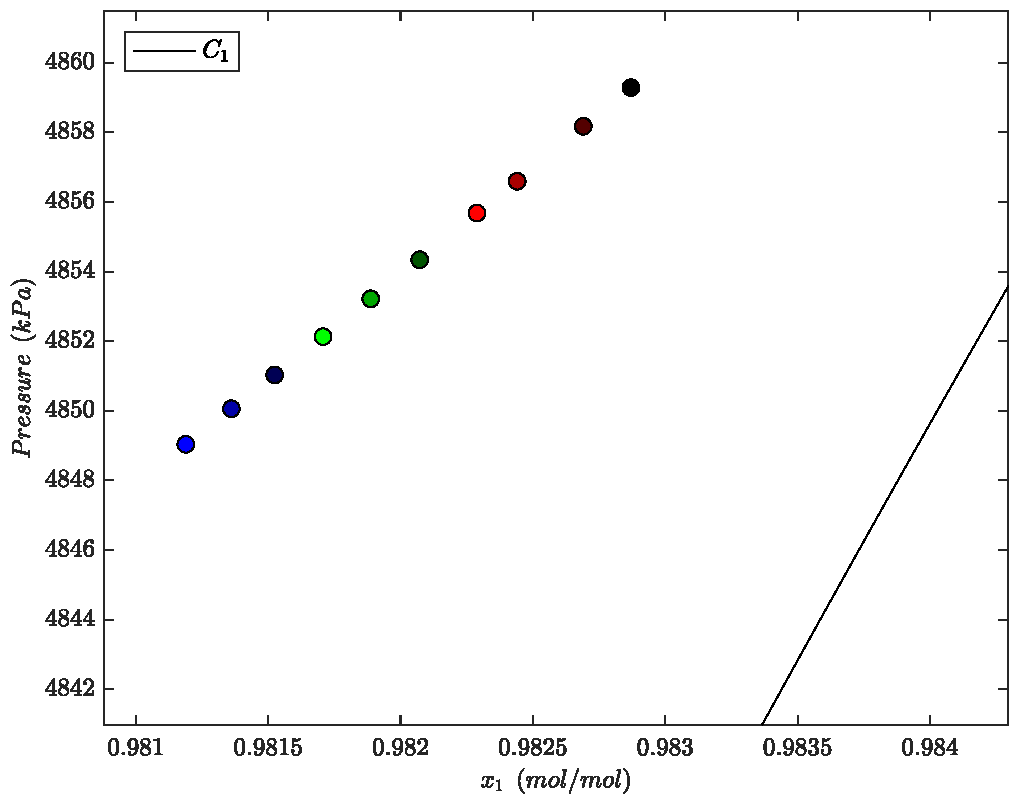
\includegraphics[width=\linewidth]{sequencia_pontos_dominio_2.pdf}
  \caption{Sequence of inverted points in the domain for root 2.}
  \label{fig:points_domain_2}
\end{subfigure}
\caption{Sequence of points that have been inverted and their respective pre-images, identified by similar colors.}
\label{fig:sequencia_inversao}
\end{figure}

Figure \ref{fig:points_image} presents the sequence of points inverted in the image. The squares in the figure are the bank of solved points. In this situation, four pre-images are observed (in accordance with the number of solutions of the original nonlinear problem). Obviously, these solutions are not roots of the original problem, since we have $ q = \left(0,0\right) $ for the physical nonlinear problem. On the other hand, as pointed previously, we maintain the same numbering of the roots (1 to 4).

The sequences of inverted points --- in the domain --- for roots 3 and 4 (high pressure roots) are represented by Figure \ref{fig:points_domain_3_4}. The end point of each of the sequences, that is, the one in which the pre-image moves closer to the critical curve (represented by the blue color), is being shown in detail by zooming. We can clearly observe the occurrence of a degeneration scenario: two solutions collapsing simultaneously to the same point of the critical curve. It should be noted that the points can be as close as desired to the critical set, which depends on the level of approximation that has been used, since the continuation method does not cross the critical curve during the inversion process. However, it is possible to estimate the point of the critical curve in the domain in which the points of each of the sequences will degenerate. Just draw a straight line which connects to each other, and check what is the intersection point between this line and the critical curve. On the other hand, Figures \ref{fig:points_domain_1} and \ref{fig:points_domain_2} contain the sequence of inverted points regarding roots 1 and 2, respectively. In these cases, the inverted points are not close to the critical curves.

Another very important factor to be considered is the positioning of the elements of each of the calculated pre-image sequences. In order for solution degeneration to occur, the degenerated points must be located on different tiles. As one point in the image approaches a critical image, two of its respective pre-images may approach a critical curve. According to \citet{malta}, the scenario that characterizes the degeneracy of solutions in pairs, as is the case of the problem studied, is that the solutions are approaching the vicinity of a critical point of the fold type. The creation of a robust bank of solved points is also essential in this analysis, since it would not be possible to calculate the correct pre-images if the inversion method took as an initial guess a point in the bank of solved points in the domain that was located on a different tile than the one in which the desired solution is.

Hereafter, we detail the inversion process for the point close to the critical image. Figure \ref{fig:L_path_image} indicates the L-shaped path in the image. Again, the square represents a point in the bank of solved points and the desired point, namely, the point to be inverted, is represented by a circle with the corresponding color. In turn, the paths in the domain are detached in Figure \ref{fig:L_path_domain}. One can note that the L-shaped paths were deformed and are virtually straight lines. This is due to the critical image of the system limiting the tile where the point to be inverted is located in a very restricted area. With this, the bank of solved points must be relatively close to the point to be inverted (besides the fact of taking the point contained in the bank that is closest to the point to be inverted as initial guess) and the method of continuation reaches the pre-image through an almost straight path. Once again, the degeneration process is clearly indicated and the critical curve has a fold at this point.

\begin{figure}
\centering
\begin{subfigure}{.48\textwidth}
  \centering
  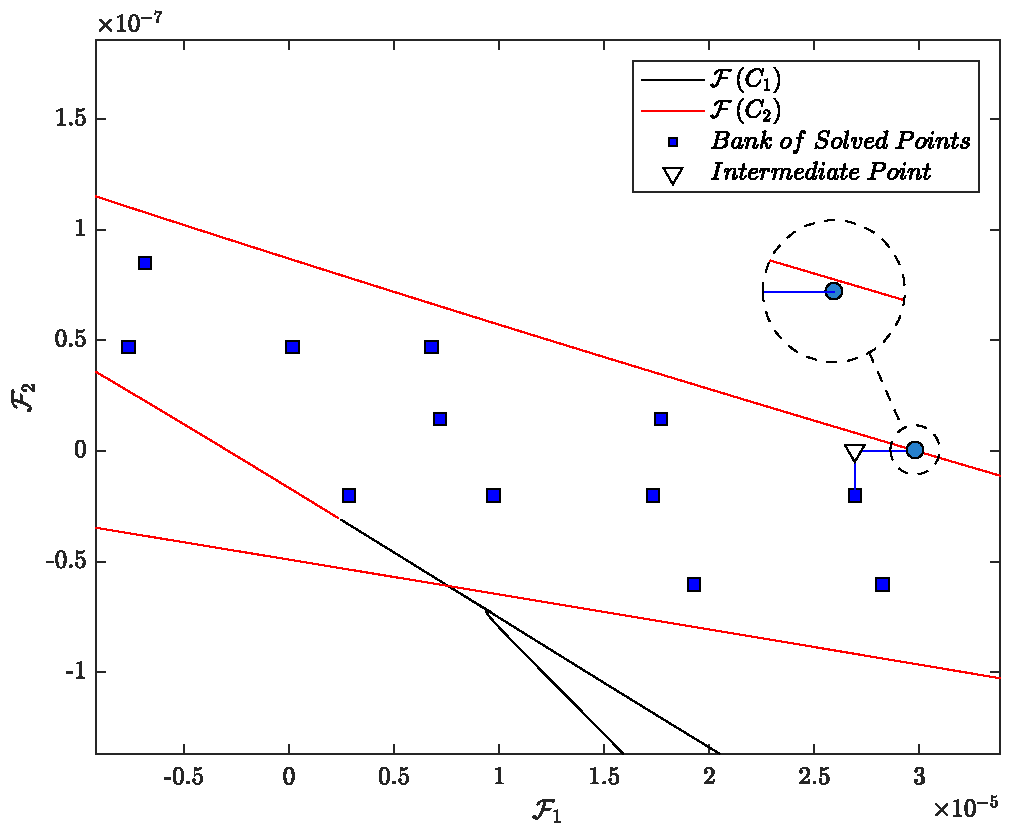
\includegraphics[width=\linewidth]{caminho_L_degeneracao_imagem_new.pdf}
  \caption{L-shaped path in the image.}
  \label{fig:L_path_image}
\end{subfigure}\hfill
\begin{subfigure}{.48\textwidth}
  \centering
  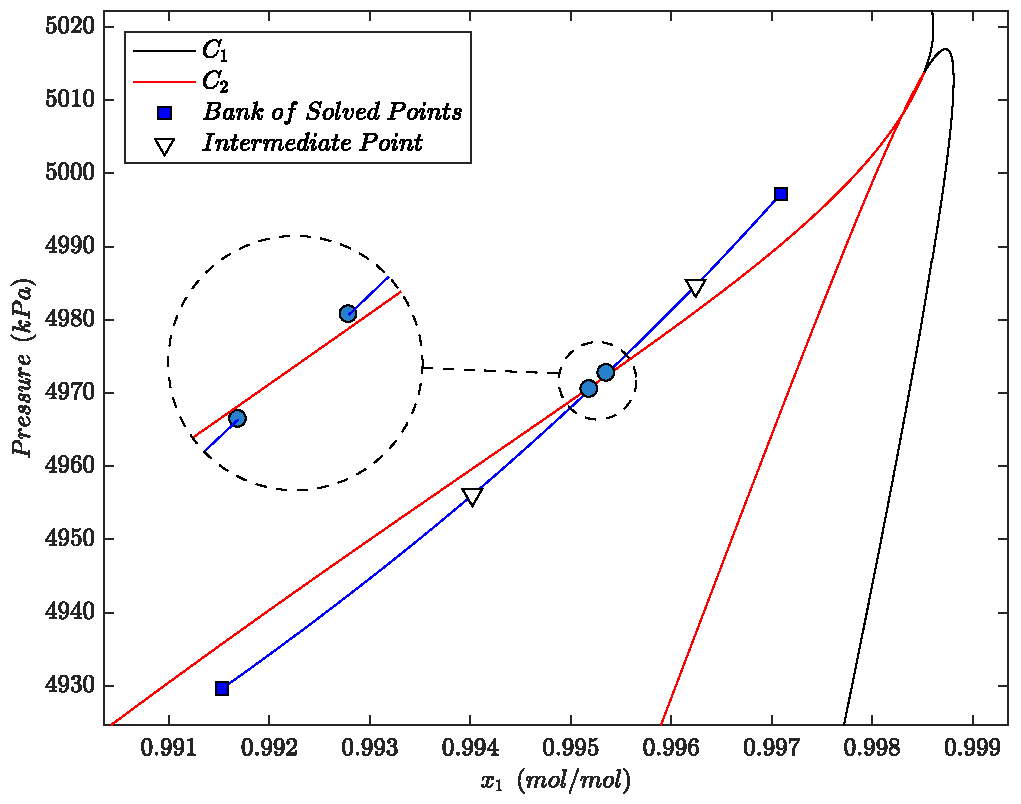
\includegraphics[width=\linewidth]{caminhos_L_degeneracao_dominio_new.pdf}
  \caption{L-shaped path in the domain for the roots 3 and 4.}
  \label{fig:L_path_domain}
\end{subfigure}
\caption{}
\label{fig:L_path_domain_image}
\end{figure}

\subsection{Results at $ T = 304.5 $ K and $ T = 280 $ K, with $ y_1 = 0.99945 $}

In the case analyzed previously, the degeneracy of two of the system solutions around a fold was clear when the point to be inverted was sufficiently close to the critical image. Now, two cases will be analyzed simultaneously, such as each of the systems, through only the variation of their temperature, presents different quantities of solutions. The objective is to show the exact moment in which the degeneration of two solutions of the problem occurs, but due to the proximity of the solutions to the critical set. Here, the same strategy of the previous case will be used to obtain the results: a sequence of points in the image will be inverted, from a known point (for instance, $ q = \left(0, 0\right) $) to a point sufficiently close to the critical image, without being crossed. Thus it is possible to observe the behavior of the solutions in the domain of the problem.

At $T = 304.5$ K and $y_1 = 0.99945$, the dew point curve still exhibits a double retrograde behavior, but now the curve has a sigmoidal shape (instead of a double dome). In this situation, we observe three dew point pressures (and liquid compositions) for a narrow range of molar fractions. This time, the system has two solutions at high pressures and one under reduced pressure. In addition, the distance between the solutions, in terms of pressure, is relatively higher than in the previous case.

\subsubsection{Inversion process --- approaching  the critical image}

Figure \ref{fig:imagem_S} shows the sequence of points in the image to be inverted, from $ q = \left(0, 0\right) $ to a point sufficiently close to the critical image. Following the same trend, the points in the image were identified by distinct colors, and their pre-images respected the established organization. The bank of solved points was randomly arranged in the image and each of its pre-images was obtained. In relation to the previous problem, it is not possible to use the same bank of solved points, since two parameters were varied, temperature and pressure, what makes the system have absolutely different thermodynamic characteristics. The zoom in Figure \ref{fig:imagem_S} shows that the blue point does not intersect or even cross the critical image.

Figure \ref{fig:domain_S} shows the behavior of each of the pre-images, for the two solutions at high pressures (roots 2 and 3), obtained through the method of inversion of functions from the plane to the plane. As expected, the behavior of the sequence of pre-images of the two solutions in question suggests that as we approach the critical image two solutions approach the critical curve until both collapse in a given point of the critical curve. This behavior characterizes the degeneracy of solutions.

It is known that, according to the definition, one of the conditions for characterizing a critical points of the fold type is that the kernel of the Jacobian matrix at the critical point does not coincide with the vector tangent to $ {\cal{C}} $ at the same point. In Figure \ref{fig:domain_S}, the critical point at which degeneration occurs is estimated and denoted by $ c_{k} $. The approximation was performed by interpolating between the sequence of pre-images and $ c_{k} $ is a point of the critical curve that was crossed by the interpolated curve. The accuracy of the $ c_{k} $ approximation is not significant, since it is conjectured that there are only folds in the vicinity of $ c_{k} $. Therefore, the kernel of the Jacobian matrix in $ c_{k} $ was obtained and, through the analysis of Figure \ref{fig:domain_S}, it is clear that this vector does not coincide with the vector tangent to $ {\cal{C}} $ in $ c_{k} $.

\begin{figure}
\centering
\begin{subfigure}{.48\textwidth}
  \centering
  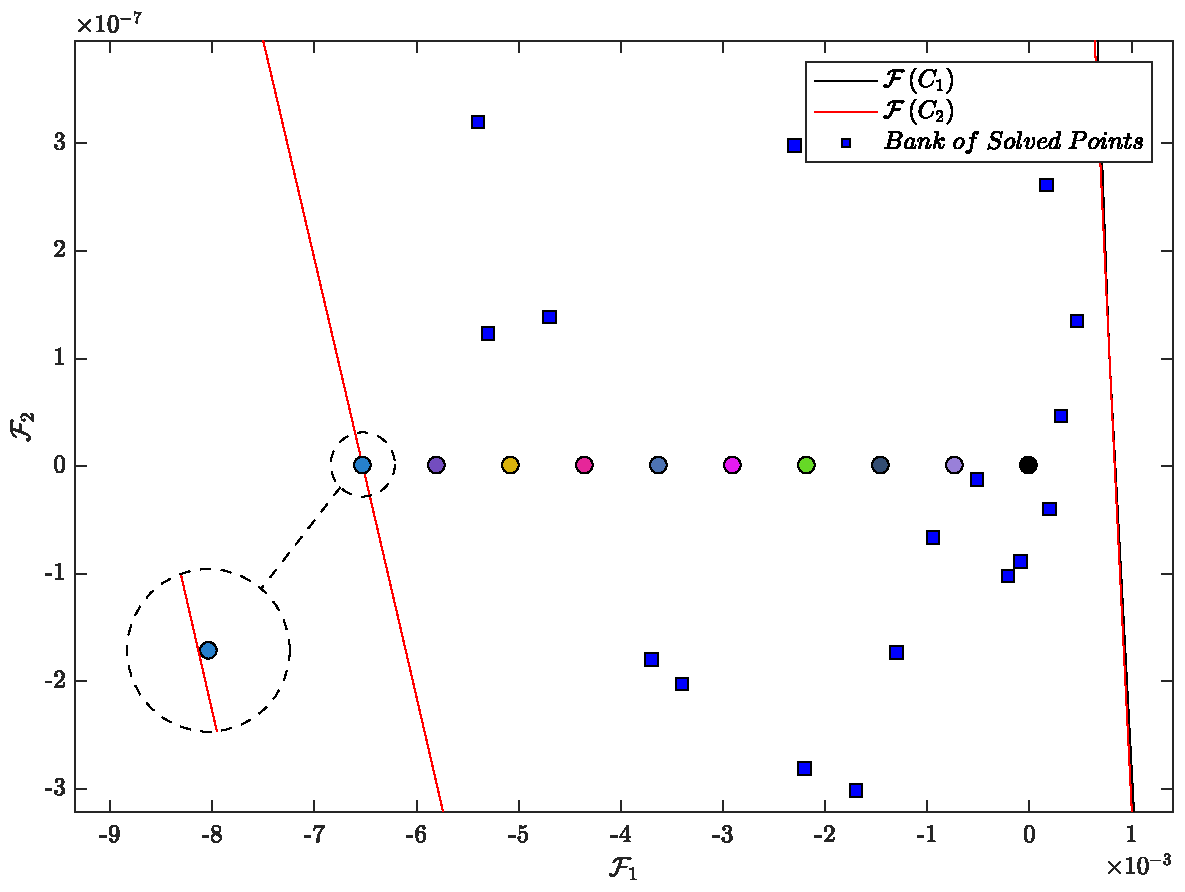
\includegraphics[width=\linewidth]{imagem3.pdf}
  \caption{Sequence of inverted points (image) for $T$ = 304.5 K and $y_1 = 0.99945$.}
  \label{fig:imagem_S}
\end{subfigure}\hfill
\begin{subfigure}{.48\textwidth}
  \centering
  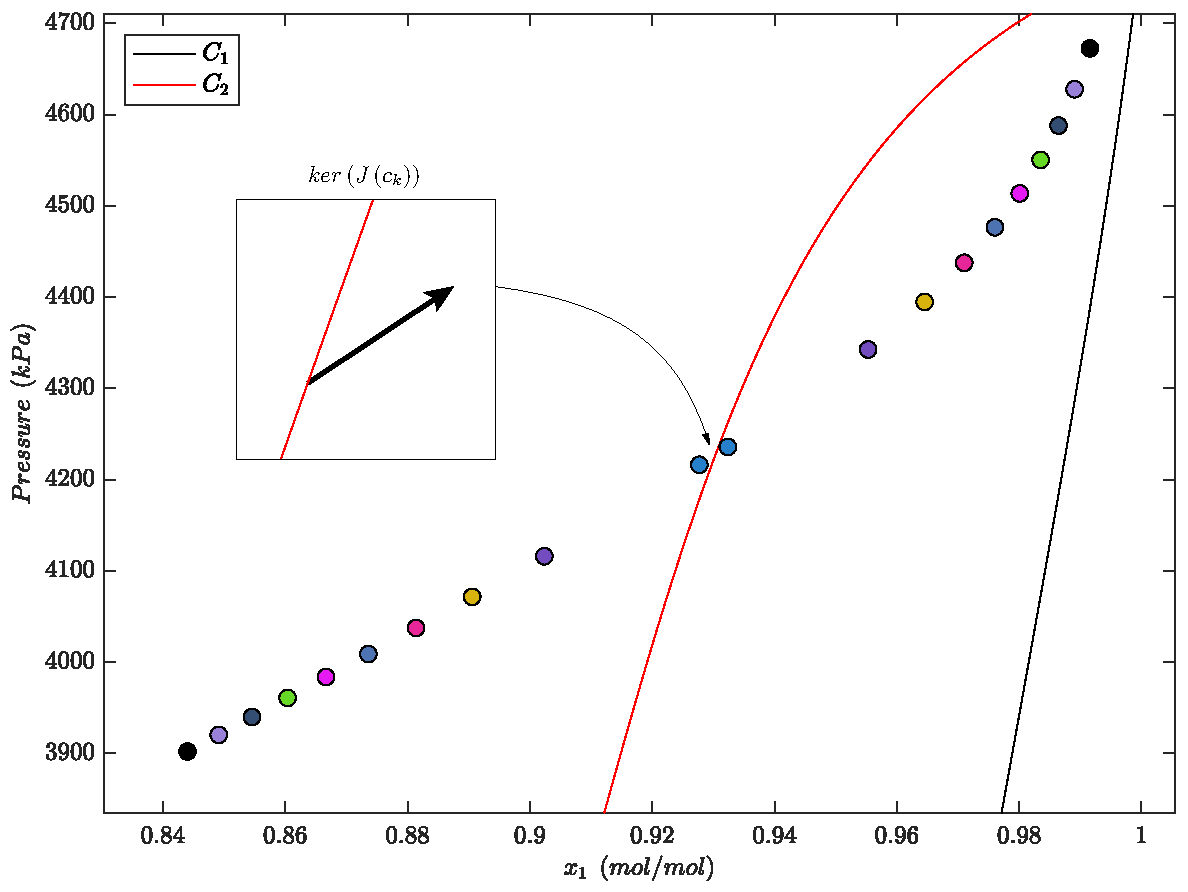
\includegraphics[width=\linewidth]{dominio3.pdf}
  \caption{Sequence of inverted points (domain) for $T$ = 304.5 K and $y_1 = 0.99945$ (Roots 2 and 3).}
  \label{fig:domain_S}
\end{subfigure}
\caption{}
\label{fig:L_path_domain_image}
\end{figure}

In turn, Figure \ref{fig:L_S} illustrates the L-shaped path of the inversion process in the domain to the last point of the sequence in the image (the one closest to the critical image, marked in blue in Figure \ref{fig:imagem_S}). Again, we observed that the two pre-images, corresponding to roots 2 and 3, tend to degenerate into a single pre-image. In addition, one can note the importance of knowing the critical set of the problem and, consequently, the tiles that form the domain of the system. They define the points of singularities that may cause problems to the continuation method in the process of creating the L-shaped path of the inversion step and consequently provide the analysis of the degeneracy of solutions.

\begin{figure}[!ht]
	\begin{center}
		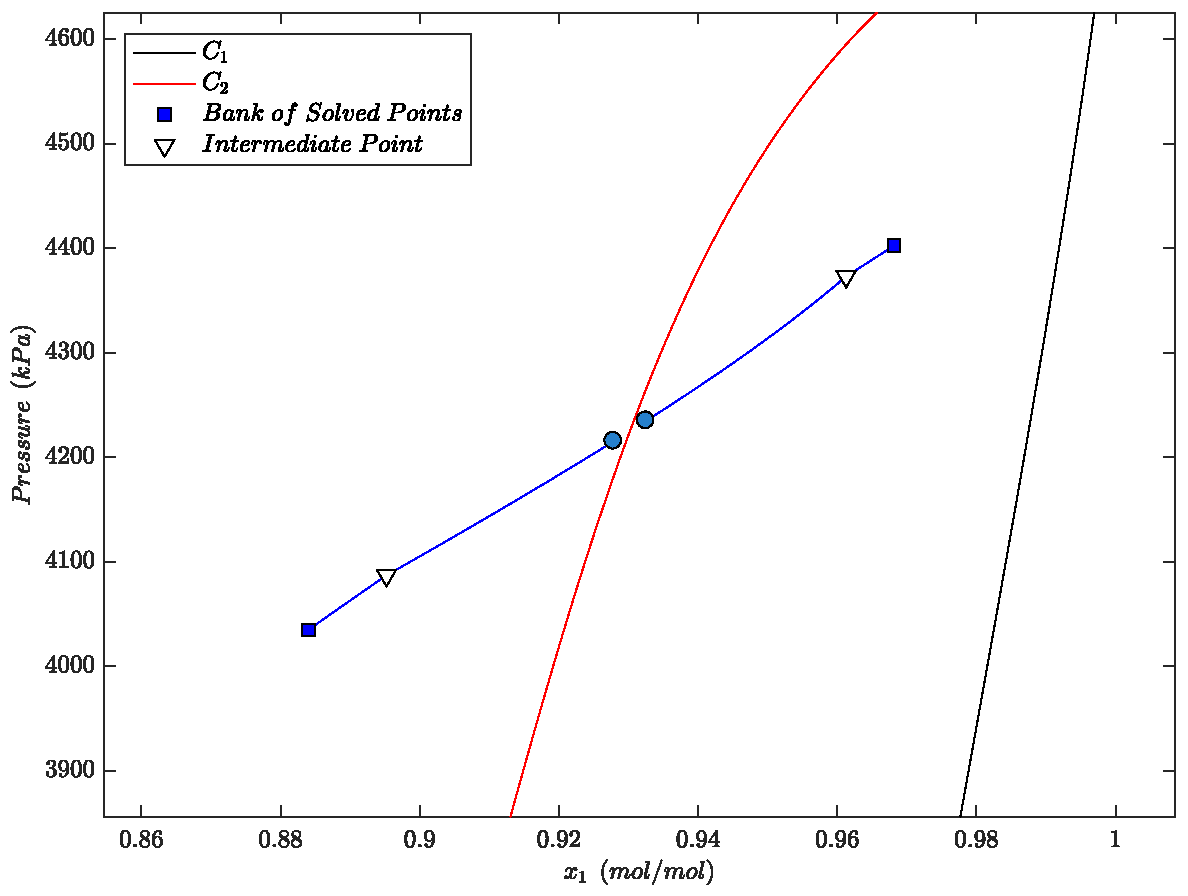
\includegraphics[scale=0.50]{caminhos_L_degeneracao_dominio2.pdf}
		\caption{The \enquote{L} path in the domain, Roots 2 and 3, for $T$ = 304.5 K and $y_1 = 0.99945$.}\label{fig:L_S}
	\end{center}
\end{figure}

The use of the bank of solved points of the previous problem would not be possible in this problem because, in addition to the number of distinct pre-images in each of the problems, possibly the points of the bank of solved points in the domain could be located in tiles different from the desired pre-images. Since the points contained in the bank act as the initial guess for the method of continuation in the inversion step, the L-shaped path would necessarily cross the critical curve of the problem, which could cause an error in the computational routine.

Finally, Figure 9 shows the L-shaped path of the problem at T = 280 K and y1 = 0.99945. Under such conditions, the problem has only one solution, despite the sigmoid behavior, as can be seen in Figure 1.

\begin{figure}[!ht]
	\begin{center}
		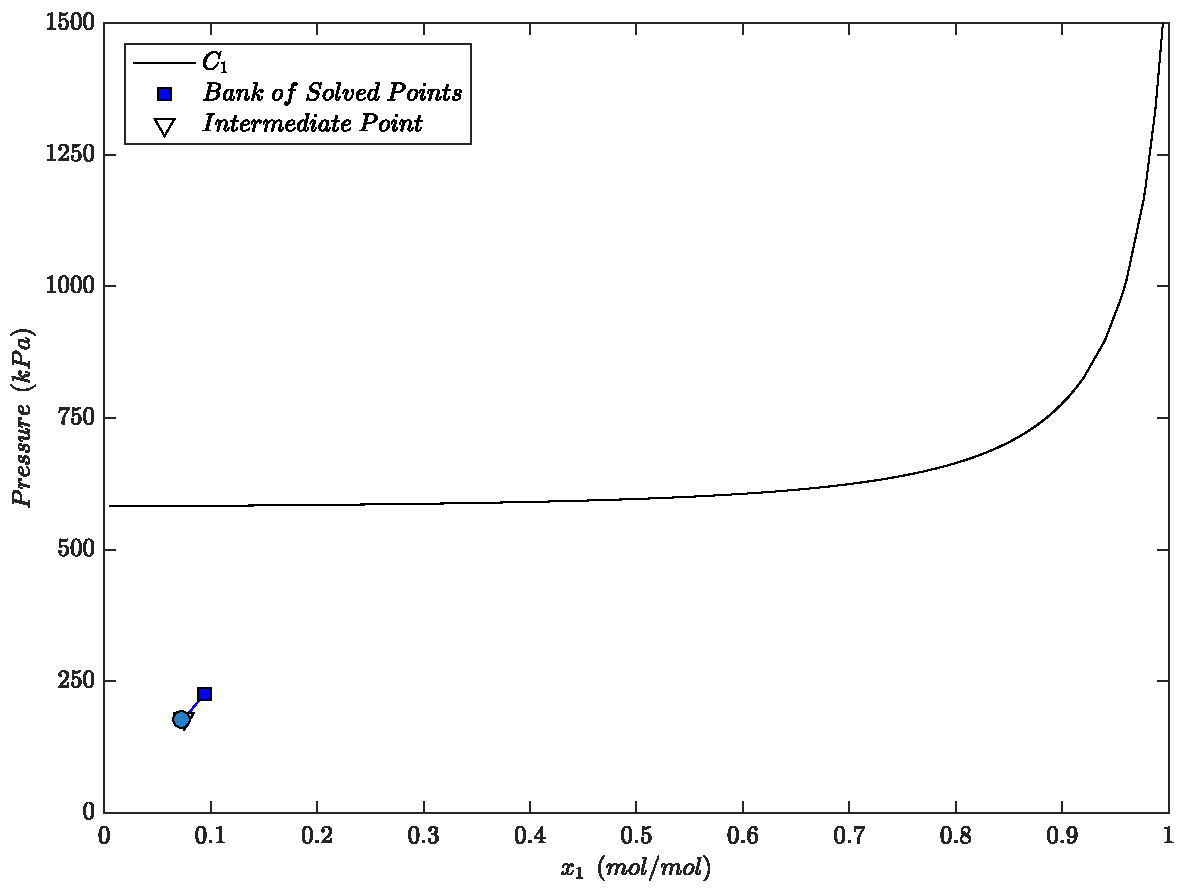
\includegraphics[scale=0.50]{caminhos_L_degeneracao_dominio3.pdf}
		\caption{The L-shaped path in the domain, Root 1, for $T$ = 280.0 K and $y_1 = 0.99945$.}\label{fig:L_S2}
	\end{center}
\end{figure}


\subsection{The influence of temperature on the critical curve}

The last resource to be investigated in this work corresponds to the influence of the system temperature (specified) on the critical curve. Obviously, the phenomenon of double retrograde vaporization is a function dependent on the temperature of the system. Since the critical curves have a direct influence on the process of obtaining pre-images --- the system solutions --- the analysis of the variation of the temperature of the system is essential in the resolution of systems of this type. The behavior of the critical curves under different values of the system parameters (in this case, the temperature) can clarify the occurrence of numerical errors in nonlinear system resolution techniques.

To perform the tests, the critical sets of the systems were obtained by fixing the molar fraction of the ethane vapor phase at $ y_{1} = 0.99966 $ and varying the system temperature from $ T = 299 $ K to $ T = 300 $ K, as can be seen in the dew point curves shown in Figure \ref{fig:bubble_curves_temeprature_variation}. In this way, it was possible to evaluate the behavior of the critical images of the system, varying only one of the parameters of the model, so that all systems analyzed had the same number of pre-images when $ q = \left(0,0\right) $.

In Figure \ref{fig:critical_images_temeprature_variation}, it is possible to observe the influence of the system temperature variation on the behavior of the critical images (and therefore the variation of the critical curves in the sense of the solutions degeneration) in the vicinities of $ q = \left(0, 0\right) $. As the temperature of the system decreases, its critical image is ever closer to $ q = \left(0, 0\right) $. The closer the critical image is to the point to be inverted, the more limited will be the performance of the numerical method used to obtain the results, since it increases the chances of crossing the critical curve.

\begin{figure}
\centering
\begin{subfigure}{.5\textwidth}
  \centering
  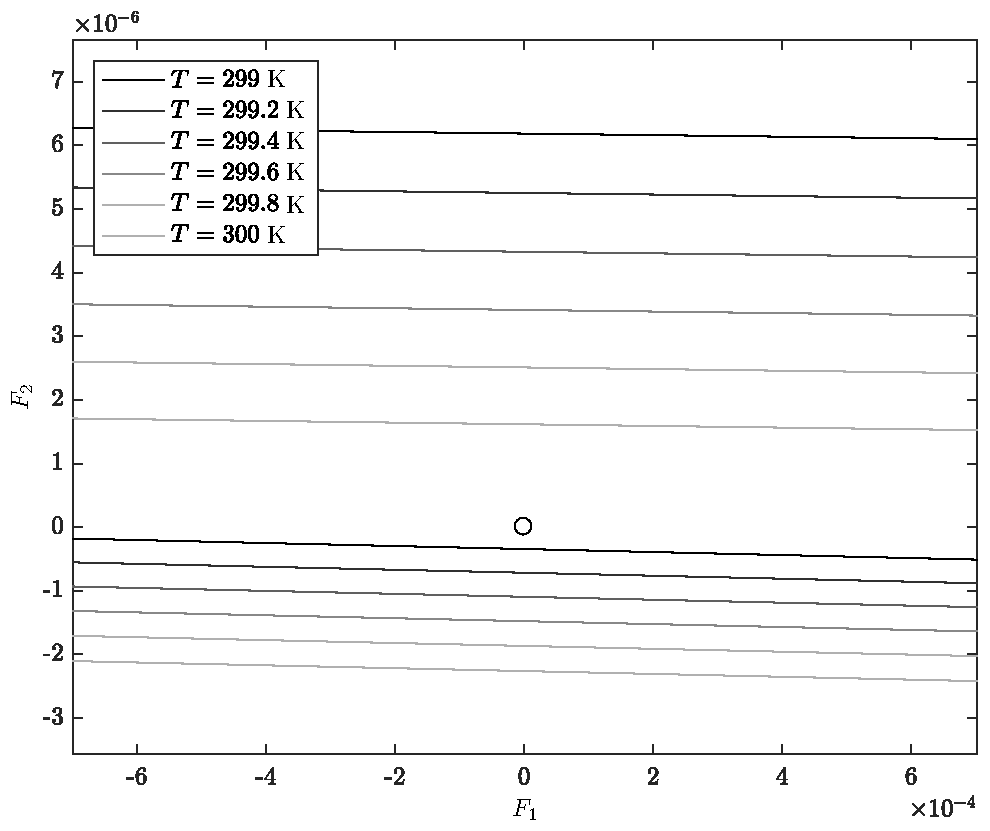
\includegraphics[width=0.95\columnwidth]{variacao_temperatura.pdf}
  \caption{Critical images for different temperatures}
  \label{fig:critical_images_temeprature_variation}
\end{subfigure}%
\begin{subfigure}{.5\textwidth}
  \centering
  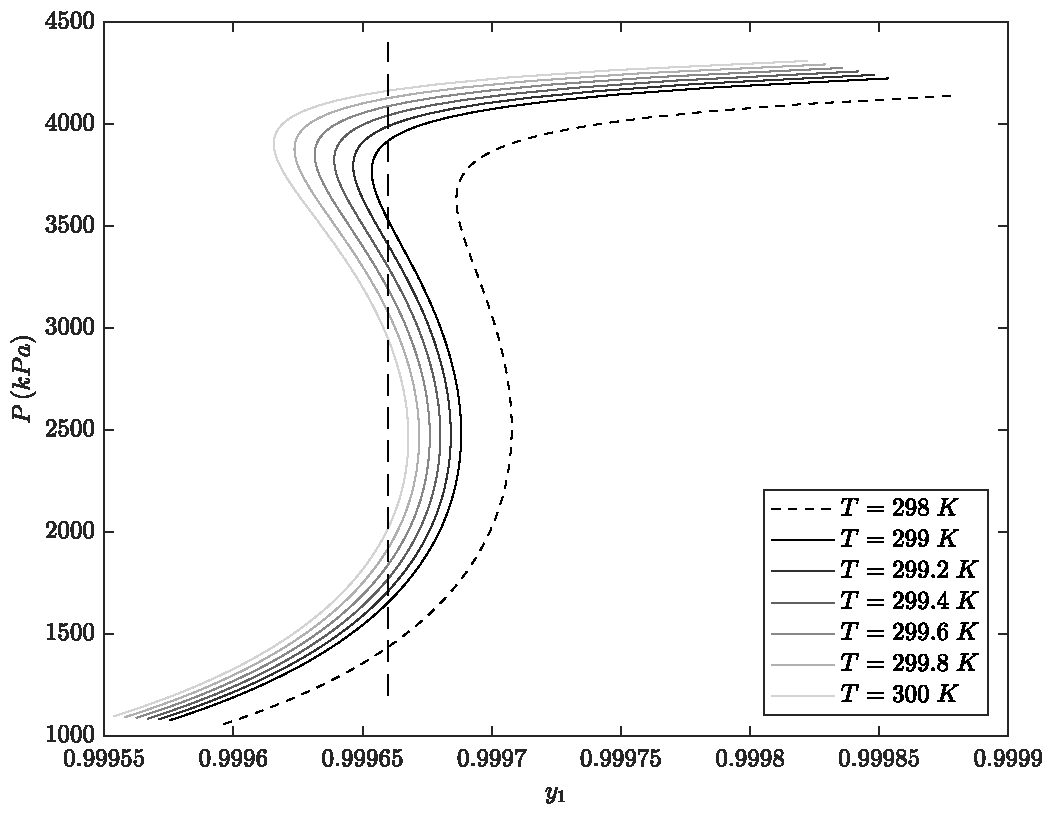
\includegraphics[width=0.95\columnwidth]{variacao_temperatura_ponto_bolha.pdf}
  \caption{Dew point curves for different temperatures}
  \label{fig:bubble_curves_temeprature_variation}
\end{subfigure}
\caption{Influence of system temperature variation on the critical images of the problem. The molar fraction of the vapor phase of ethane is set at $ y_1 = 0.99966 $ for all cases, as shown in the dashed line.}
\label{fig:domain_image_r}
\end{figure}

When the molar fraction of the vapor phase of ethane is fixed, the system obviously no longer has three distinct solutions, in the case studied, when defining a temperature that carries a behavior like that shown by the dew point curve calculated at $ T = 298 $ K in Figure \ref{fig:bubble_curves_temeprature_variation}. However, the case treated here predicts that, for a given system temperature, a certain segment of the critical image may be so close to $ q = \left(0, 0\right) $ that it would be very difficult to obtain the pre-images of the system if the derivatives were evaluated sufficiently close to the point where the pre-images are desired.

\begin{figure}[!ht]
\centering
\begin{subfigure}{.48\textwidth}
  \centering
  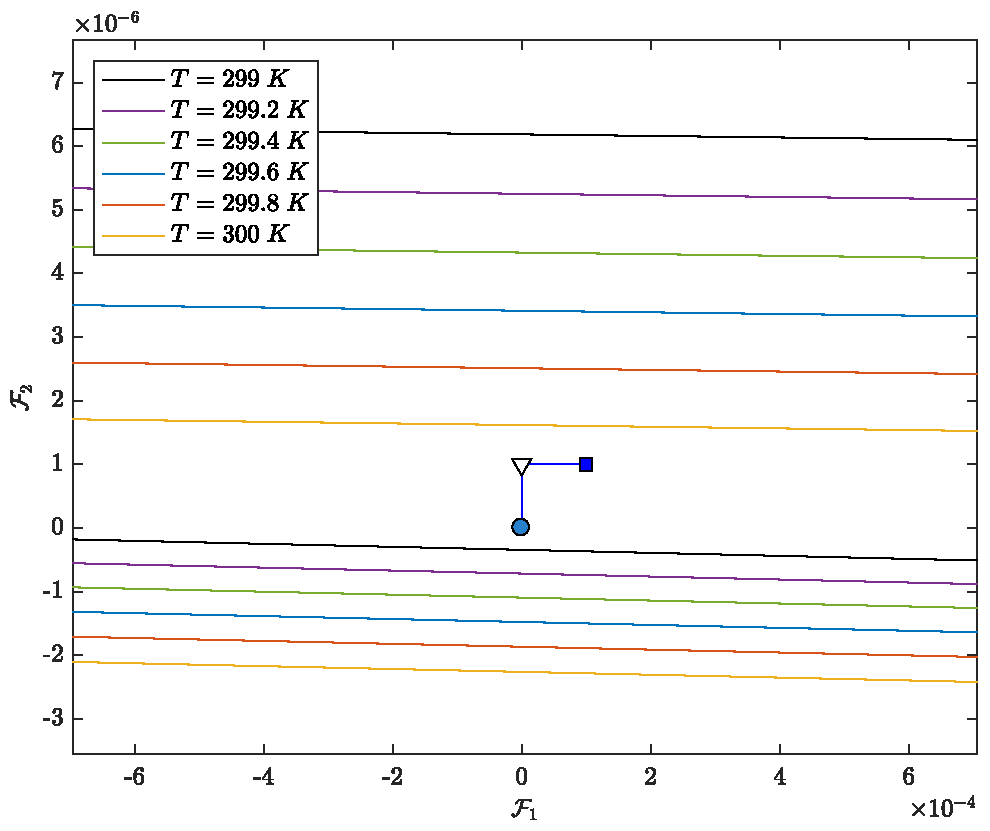
\includegraphics[width=\linewidth]{caminho_L_imagem_unico_banco.pdf}
  \caption{L-shaped path in the image for the inversion of all points using the same bank of solved points.}
  \label{fig:unique_bank_image}
\end{subfigure}\hfill
\begin{subfigure}{.48\textwidth}
  \centering
  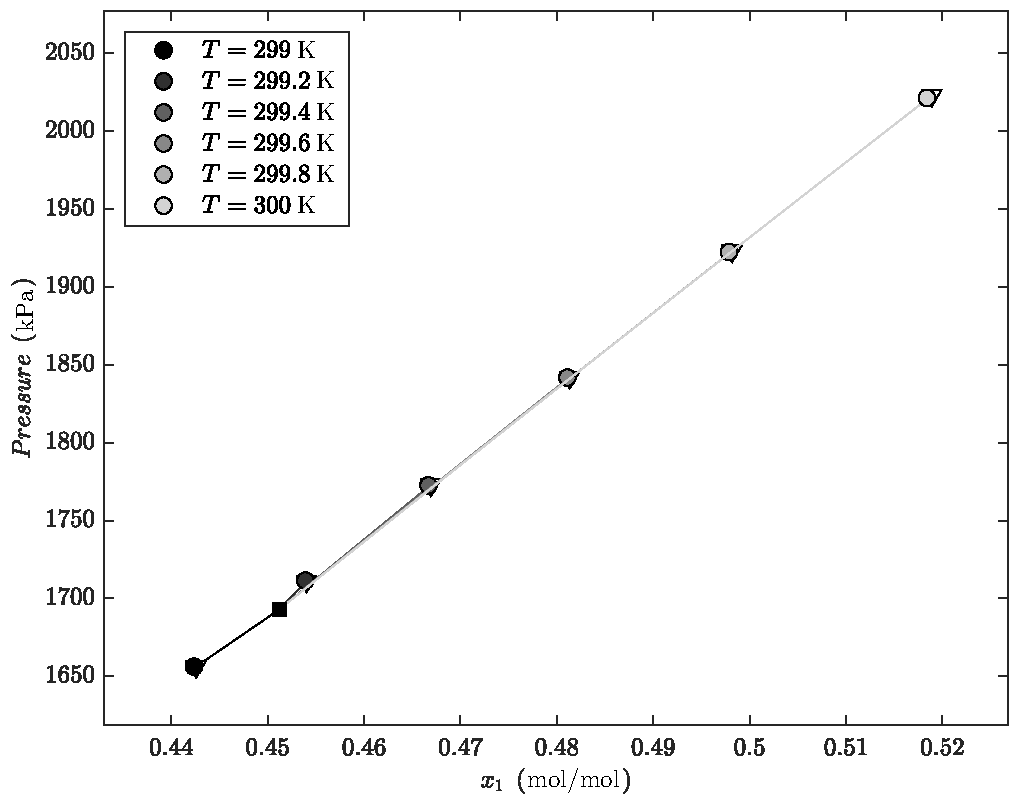
\includegraphics[width=\linewidth]{caminhos_L_dominio_unico_banco1.pdf}
  \caption{L-shaped paths in the domain referring to root 1 of each of the systems.}
  \label{fig:unique_bank_root_1}
\end{subfigure}\\
\begin{subfigure}{.48\textwidth}
  \centering
  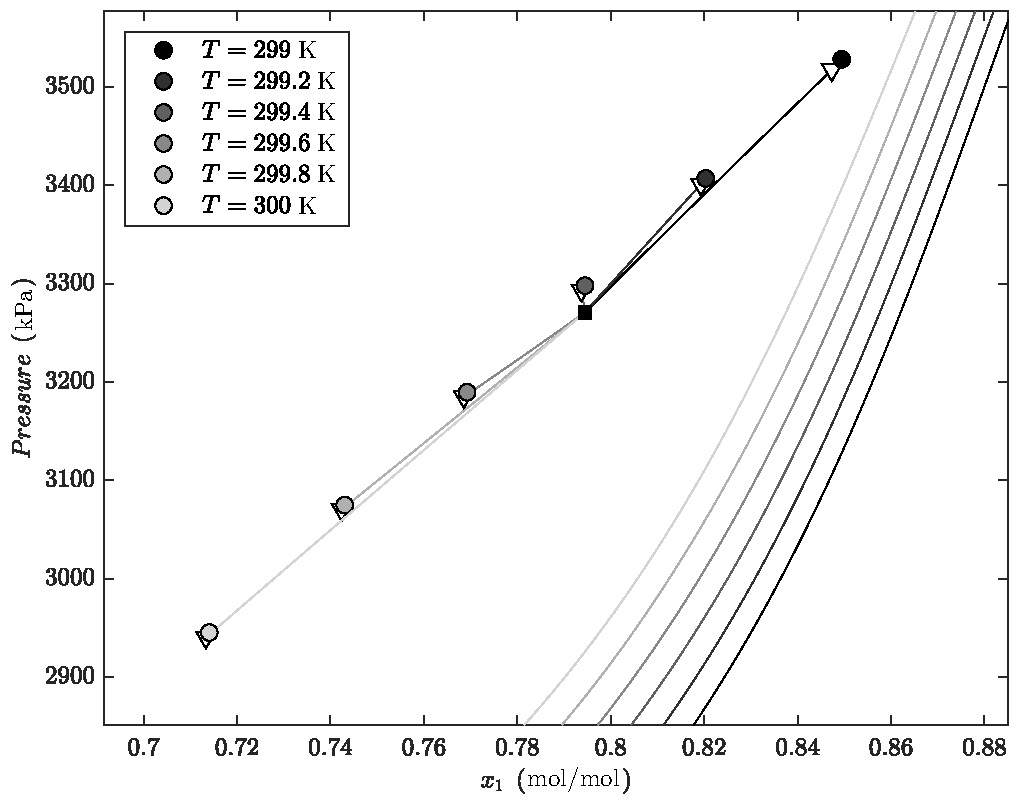
\includegraphics[width=\linewidth]{caminhos_L_dominio_unico_banco2.pdf}
  \caption{L-shaped paths in the domain referring to root 2 of each of the systems.}
  \label{fig:unique_bank_root_2}
\end{subfigure}\hfill
\begin{subfigure}{.48\textwidth}
  \centering
  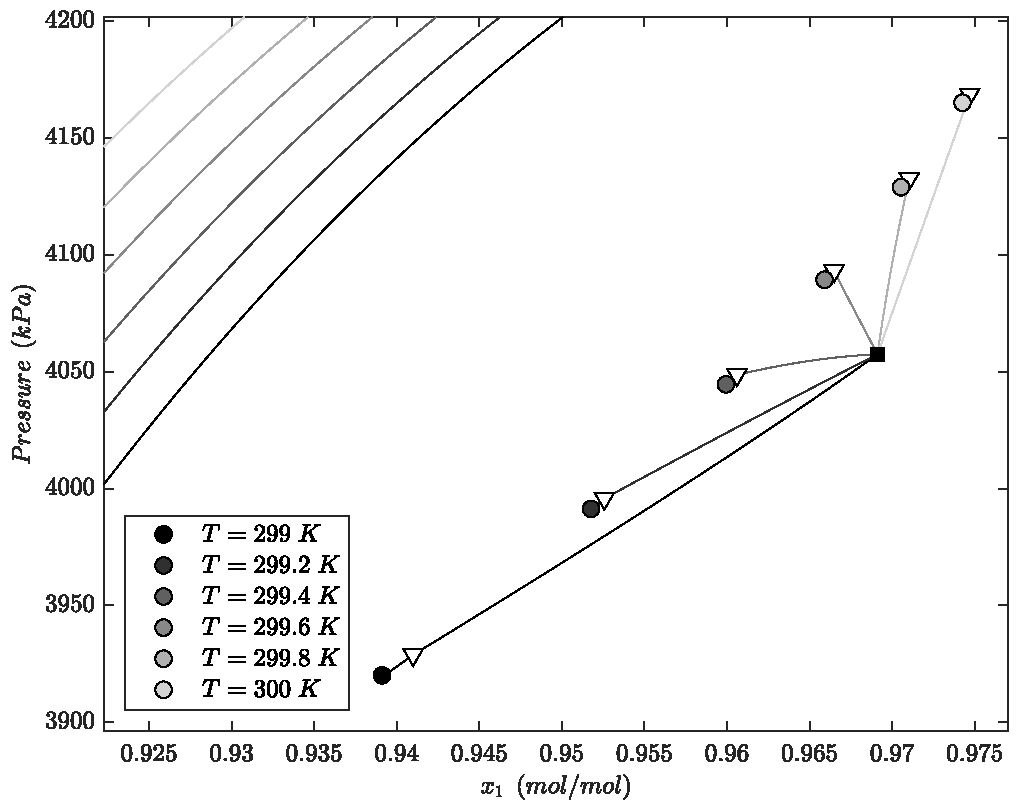
\includegraphics[width=\linewidth]{caminhos_L_dominio_unico_banco3.pdf}
  \caption{L-shaped paths in the domain referring to root 3 of each of the systems.}
  \label{fig:unique_bank_root_3}
\end{subfigure}
\caption{All solutions of the systems varying from $ T = 299 $ K to $ T = 300 $ K, with $ y_{1} = 0.99966 $, using the same bank of solved points, obtained for the system at $ T = 299 $ K.}
\label{fig:sequencia_inversao}
\end{figure}

\section{Conclusions}

It was observed that, at least in the cases studied, degenerate solutions were always those with the highest pressure value. This tendency occurs because, in general, the higher pressure solutions are more unstable (from a mathematical point of view). Particularly during the occurrence of the double-dome phenomenon of double retrograde vaporization, the upper dome occurs under a very narrow range of molar fraction and pressure in the vicinity of high pressure solutions. Under small variations of the system temperature, the double dome ceases to exist and the dew point curve takes the sigmoidal form. This fact explains the occurrence of degeneration of solutions that are usually at high pressures.

%%%%%%%%%%%%%%%%%%%%%%%%%%%%%%%%%%%%%%%%%%%%%%%%%%%%%%%%%%%%%%%%%%%%%
%% The "Acknowledgement" section can be given in all manuscript
%% classes.  This should be given within the "acknowledgement"
%% environment, which will make the correct section or running title.
%%%%%%%%%%%%%%%%%%%%%%%%%%%%%%%%%%%%%%%%%%%%%%%%%%%%%%%%%%%%%%%%%%%%%
\begin{acknowledgement}

The authors thank to the Brazilian agencies Coordination for the Improvement of Higher Education Personnel (CAPES) and the Carlos Chagas Filho Foundation for Research Support in the State of Rio de Janeiro (FAPERJ) for providing partial financial support to conduct this research.

\end{acknowledgement}

%%%%%%%%%%%%%%%%%%%%%%%%%%%%%%%%%%%%%%%%%%%%%%%%%%%%%%%%%%%%%%%%%%%%%
%% The appropriate \bibliography command should be placed here.
%% Notice that the class file automatically sets \bibliographystyle
%% and also names the section correctly.
%%%%%%%%%%%%%%%%%%%%%%%%%%%%%%%%%%%%%%%%%%%%%%%%%%%%%%%%%%%%%%%%%%%%%
\bibliography{achemso-demo}

\end{document}
